\documentclass[a4paper,14pt]{extarticle}
\usepackage{color}
\usepackage{amsmath}
\usepackage{amsthm}
\usepackage{amssymb}
\usepackage{bbold}
\usepackage{mathtools}
\usepackage{centernot}
\usepackage{tikz}
\usepackage{tikz-cd}
\usepackage{caption}
\usepackage{adjustbox}
\usepackage{multicol}  

\theoremstyle{definition}
\newtheorem*{theorem}{Theorem}
\newtheorem*{definition}{Definition}
\newtheorem*{lemma}{Lemma}
\newtheorem*{corollary}{Corollary}
\newtheorem*{proposition}{Proposition}
\newtheorem*{eg}{Example}
\newtheorem*{remark}{Remark}

\begin{document}


\title{\textbf{Algebraic Topology - MATH0023}}
\author{\textbf{Based on lectures by Prof FEA Johnson}\\ Notes taken by Imran Radzi}
\date{}
\maketitle

\pagenumbering{roman}
Notes based on the Autumn 2021 Algebraic Topology lectures by Prof FEA Johnson.
\begingroup
\let\cleardoublepage\clearpage
\tableofcontents
\endgroup
\newpage
\pagenumbering{arabic}

\vspace{12pt}

\section{Simplicial complexes}

\begin{definition}[Simplicial complex]
	A \emph{simplicial complex} $X$ is a pair $(V_X,\mathcal{S}_X)$ where $V_X$ denotes the vertex set of $X$ and $\mathcal{S}_X$ is the set of
	\textit{finite, non-empty} subsets of $V_X$ satisfying
	\begin{enumerate}
		\item $\forall v\in V_X$, then $\{v\}\in\mathcal{S}_X$
		\item If $\sigma\in\mathcal{S}_X, \,\tau\subset\sigma, \,\tau\neq\emptyset$, then $\tau\in\mathcal{S}_X$. 
	\end{enumerate}
	$\mathcal{S}_X$ is called the set of \textit{simplices} of $X$.
\end{definition}

\begin{eg}
	A \emph{standard 1-simplex}, denoted by $\Delta^1$ is simply the line segment (or usually denoted by $I$). 
	\[V_{\Delta^1}=\{0,1\}\] \[\mathcal{S}_{\Delta^1}=\{\{0\},\{1\},\{0,1\}\}\]
	\begin{center}
	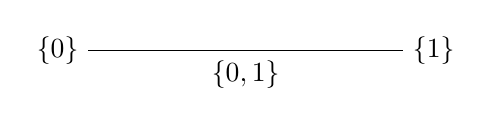
\begin{tikzpicture}
		\draw (-2,0) node[left] {$\{0\}$} node[midway,below] {$\{0,1\}$} -- (2,0) node[right] {$\{1\}$} ;
	\end{tikzpicture}
	\end{center}

\vspace{12pt}

	A \emph{standard 2-simplex}, denoted by $\Delta^2$ is the equilateral triangle.
	\[V_{\Delta^2}=\{0,1,2\}\] \[\mathcal{S}_{\Delta^2}=\{\{0\},\{1\},\{2\},\{0,1\},\{0,2\},\{1,2\},\{0,1,2\}\}\]
	\begin{center}
	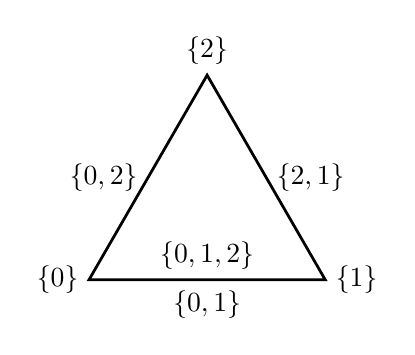
\begin{tikzpicture}
		 \draw [line width=1pt] (0,0) node[left] {$\{0\}$} -- (60:3) node[above] {$\{2\}$}  node[midway,left] {$\{0,2\}$}
		-- (3,0) node[right] {$\{1\}$} node[midway,right] {$\{2,1\}$} -- cycle node[midway,below] {$\{0,1\}$} node[midway, above]{$\{0,1,2\}$};
	\end{tikzpicture}
	\end{center}

	In general, the \emph{standard $n$-simplex} $\Delta^n$, is $\Delta^n=(V_{\Delta^n},\mathcal{S}_{\Delta^n})$ where
	\[V_{\Delta^n}=\{0,1,\ldots,n\}\] \[\mathcal{S}_{\Delta^n}=\{\alpha:\alpha\subset\{0,\ldots,n\}, \,\alpha\neq\emptyset\}\]
\end{eg}

\vspace{12pt}

\noindent If $X=(V_x,\mathcal{S}_X)$ is a simplicial complex, we now want to pick a field $\mathbb{F}$, usually $\mathbb{Q}$ or $\mathbb{F}_2$ (in this course) and want to produce a sequence of vector 
spaces (over $\mathbb{F}$)

\[C_n(X)_{0\leq n}\]

$C_0(X)$ is the vector space whose basis elements are simply the vertices of the simplicial complex, and this has dimension 0.

\begin{definition}[$k$-simplex of a simplicial complex]
	If $X$ is a simplicial complex then a \emph{$k$-simplex of $X$} is a simplex $\sigma\in\mathcal{S}_X$ such that $|\sigma|=k+1$.
\end{definition}

\noindent $C_k(X)$ is the vector space whose basis elements are the \emph{oriented} $k$-simplices of $X$ which are the following symbols,
\[[v_0,v_1,\ldots,v_n]\] (where  $\{v_0,\ldots,v_n\}$ is an $n$-simplex of $X$) subject to the rules \[[v_{\rho(0)},v_{\rho(1)},\ldots,v_{\rho(n)}]=\text{sign}(\rho)[v_0,\ldots,v_n]\]

\begin{definition}
	\[\partial_n:C_n(X)\rightarrow C_{n-1}(X)\] is a linear map defined on basis elements as follows;
	\[\partial_n[v_0,\ldots,v_n]=\sum_{r=0}^n(-1)^r[v_o,\ldots,\hat{v_r},\ldots,v_n]\] where $\hat{v_r}$ indincates omission of $v_r$.
\end{definition}

\begin{eg}
	\[\partial_2[0,1,2]=[1,2]-[0,2]+[0,1]\]
	\[\partial_1[v_0,v_2]=[v_1]-[v_0]\]
	\begin{eqnarray*}
		\partial_1\partial_2[0,1,2]&=&\partial_1([1,2]-[0,2]+[0,1]) \\
					&=&([2]-[1])-([2]-[0])+([1]-[0]) \\
					&=&0
	\end{eqnarray*}
\end{eg}

\begin{proposition}[Poincaré lemma]
	Let $X$ be a simplicial complex. Consider \[\partial_r:C_r(X)\rightarrow C_{r-1}(X)\] for $r\geq1$, then \[\partial_{n-1}\partial_n\equiv 0\]
\end{proposition}

\begin{proof}
	\begin{eqnarray*}
		\partial_n[v_0,\ldots,v_n]=\sum_{r=0}^n(-1)^r[v_0,\ldots,\hat{v_r},\ldots,v_n]
	\end{eqnarray*}

	\begin{eqnarray*}
		\partial_{n-1}[v_0,\ldots,\hat{v_r},\ldots,v_n]&=&\sum_{s<r}(-1)^s[v_0,\ldots,\hat{v_s},\ldots,\hat{v_r},\ldots,v_n] \\
									&&+\sum_{s>r}(-1)^{s-1}[v_0\ldots,\hat{v_r},\ldots,\hat{v_s},\ldots,v_n]
	\end{eqnarray*}

	\begin{eqnarray*}
		\partial_{n-1}\partial_n[v_0,\ldots,v_n]&=&\sum_{s<r}(-1)^{r+s}[v_0,\ldots,\hat{v_s},\ldots,\hat{v_r},\ldots,v_n] \\
								&&+\sum_{s>r}(-1)^{r+s-1}[v_0,\ldots,\hat{v_r},\ldots,\hat{v_s},\ldots,v_n] \\
								&=&0
	\end{eqnarray*}
\end{proof}

\begin{proposition}
	If \[C_{n+1}\xrightarrow{\partial_{n+1}}C_n\xrightarrow{\partial_n}C_{n-1}\] then \[\text{im}(\partial_{n+1})\subset\ker(\partial_n)\]
\end{proposition}

\begin{proof} By previous lemma.
\end{proof}

\section{Homology}
\subsection{Quotient spaces}
Let $V$ be a vector space over a field $\mathbb{F}$, and $U\subset V$ a vector subspace.

\begin{definition}
The following set \[x+U=\{x+u:u\in U\}\] is called the (left) coset of $U$ in $V$. Note that \[x+U=x'+U\iff x-x'\in U\]	
\end{definition}

\begin{definition}[Quotient space]
	The quotient space $V/U$ is the set \[V/U=\{x+U:x\in V\}\] where addition and scalar multiplication is defined by \[(x+U)+(y+U)=x+y+U\]\[\lambda\cdot(x+U)=\lambda x+U\] and 0 is
	represented by \[0+U\] Note that $V/U$ is a vector space.
\end{definition}

\begin{proposition}
	\[\dim(V/U)=\dim(V)-\dim(U)\]
\end{proposition}

\begin{proof}
	There exists a natural linear map \[\eta:V\rightarrow V/U\] given by \[\eta(x)=x+U\] Clearly this map is surjective so \[\dim(V/U)=\dim(\text{im}(\eta))\] Now,
	\begin{eqnarray*}
		\ker(\eta)&=&\{x\in V:\eta(x)=U\}\\
			&=&\{x\in V:x+U=U\}
	\end{eqnarray*}
	and \[x+U=U\iff x-0\in U\iff x\in U\] so $\ker(\eta)=U$. Then, \[\dim(V)=\dim\ker(\eta)+\dim\text{im}(\eta)\] so \[\dim(V/U)=\dim\text{im}(\eta)=\dim(V)-\dim(U)\]
\end{proof}

\begin{definition}
	\[H_n(X;\mathbb{F})=\ker(\partial_n)/\text{im}(\partial_{n+1})\]
\end{definition}

We call $H_n(X;\mathbb{F}$) the \emph{$n^{\text{th}}$ homology group} of $X$ with coefficients in $\mathbb{F}$. If $\mathbb{F}=\mathbb{Q}$, then $\dim H_n(X;\mathbb{Q})$ is called
the $n^{\text{th}}$ \emph{Betti} number of $X$. \\

Consider $\Delta^3$. The set $\{0,1,2,3\}$ represents the 'middle' of the tetrahedron (inside, interior). If we exclude the middle and simply take its boundary, we have \[\partial\Delta^n=S^{n-1}\]
It happens that $S^2$ (middle excluded) is the simplest simplicial model of the 2-sphere.

\begin{eg}
Consider \[H_k(S^2;\mathbb{F})\] Note that \[C_n(S^2)=0\text{ for }n\geq3\] as there are no 3-simplices, so we only have to worry about
\[H_2(S^2;\mathbb{F}),H_1(S^2;\mathbb{F}),H_0(S^2;\mathbb{F})\] We proceed to calculate these from first principles. First note that $C_3(S^2)=0$. Now, (noting the order of these bases)
 $C_2(S^2)$ has basis
\[[0,1,2],[0,1,3],[0,2,3],[1,2,3]\] $C_1(S^2)$ has basis \[[0,1],[0,2],[0,3],[1,2],[1,3],[2,3]\] and lastly $C_0(S^2)$ has basis \[[0],[1],[2],[3]\]
The linear maps \[\partial_2:C_2(S^2)\rightarrow C_1(S^2)\]\[\partial_1:C_1(S^2)\rightarrow C_0(S^2)\] can both be represented by a $6\times4$ matrix and a $4\times6$ matrix respectively.

We apply $\partial_2$ and $\partial_1$ to the bases to obtain the entries to the matrices, so for example \[\partial_2([0,1,2])=[1,2]-[0,2]+[0,1]\] so the first column of the matrix representing 
$\partial_2$ is $\begin{pmatrix}1\\-1\\0\\1\\0\\0\end{pmatrix}$ Proceeding, we will obtain that
\[\partial_2=\begin{pmatrix}1&1&0&0\\-1&0&1&0\\0&-1&-1&0\\1&0&0&1\\0&1&0&-1\\0&0&1&1\end{pmatrix}\]
\[\partial_1=\begin{pmatrix}-1&-1&-1&0&0&0\\1&0&0&-1&-1&0\\0&1&0&1&0&-1\\0&0&1&0&1&1\end{pmatrix}\]
Notice that $\partial_1\partial_2=0$, which further confirms the lemma from before. Now reducing both the matrices to row reduced echelon form, we obtain
\[\begin{pmatrix}1&0&0&1\\0&1&0&-1\\0&0&1&1\\0&0&0&0\\0&0&0&0\\0&0&0&0\end{pmatrix}\] thus $\dim\ker\partial_2=1,\,\dim\text{im }\partial_2=3$
\[\begin{pmatrix}1&0&0&-1&-1&0\\0&1&0&1&0&-1\\0&0&1&0&1&1\\0&0&0&0&0&0\end{pmatrix}\] thus $\dim\ker\partial_1=3,\,\dim\text{im }\partial_1=3$
\[0\xrightarrow[\partial_3]{} C_2\xrightarrow{\partial_2}C_1\xrightarrow{\partial_1} C_0\rightarrow0\]
so now \[H_2(S^3)=\ker(\partial_2)/\text{im}(\partial_3)=\ker(\partial_2)\cong\mathbb{F}\] as $\text{im}(\partial_3)=0$, so in total, \[H_2(S^2;\mathbb{F})\cong\mathbb{F}\] Next,
\[H_1(S^2)=\ker(\partial_1)/\text{im}(\partial_2)\] Now note that \[\dim H_1(S^2)=\dim\ker(\partial_1)-\dim\text{im}(\partial_2)=3-3=0\] thus \[H_1(S^2;\mathbb{F})=0\] Next,
\[H_0(S^2)=\ker(\partial_0)/\text{im}(\partial_1)=C_0/\text{im}(\partial_1)\] and \[\dim H_0(S^2)=\dim C_0-\dim\text{im}(\partial_1)=4-3=1\] thus \[H_0(S^2;\mathbb{F})\cong\mathbb{F}\]
\end{eg}

We've shown
\[ H_k(S^2;\mathbb{F})\begin{cases} 
			      \mathbb{F} & k=0 \\
			      0 & k=1 \\
			      \mathbb{F} & k=2 \\
			      0 & k\geq3
			   \end{cases}
\]

We will soon see that this theorem generalises if \[S^n=\Delta^{n+1}\] then \[H_k(S^n)=\begin{cases}\mathbb{F}&k=0,n\\0&\text{otherwise}\end{cases}\]

\subsection{Chain complex}
\begin{definition}[Chain complex]
	Let $\mathbb{F}$ be a field. A \emph{chain complex} over $\mathbb{F}$ is \[C_*=(C_r,\partial_r)_{r\in\mathbb{N}}\] where
	\begin{enumerate}
		\item Each $C_r$ is a vector space over $\mathbb{F}$
		\item $\partial_r:C_r\rightarrow C_{r-1}$ is a linear map such that $\partial_r\partial_{r+1}=0$ for all $r$.
	\end{enumerate}
\end{definition}

If $X=(V_X,\mathcal{S}_X)$, we have defined a chain complex \[C_*(X)=(C_r(X),\partial_r)\]

Given a chain complex \[C_*(C_r,\partial_r)_{r\geq0}\] we define its \emph{homology} $H_*(C_*)$ by \[H_k(C_*)=\ker(\partial_k)/\text{im}(\partial_{k+1})\]

If $X=(V_X,\mathcal{S}_X)$ is a simplicial complex, we define \[H_k(X;\mathbb{F})=H_k(C_*(X;\mathbb{F}))\]

\subsection{Simplicial mapping}
\begin{definition}[Simplicial mapping]
	Let $X,Y$ be simplicial complexes, i.e., $X=(V_X,\mathcal{S}_X)$ and $Y=(V_Y,\mathcal{S}_Y$). A \emph{simplicial mapping} $f:X\rightarrow Y$ is a mapping of vertex sets
	$f:V_X\rightarrow V_Y$ such that \[\sigma\in\mathcal{S}_X\implies f(\sigma)\in\mathcal{S}_Y\]
\end{definition}

\begin{eg}
	Let $X=Y=\Delta^2$. Then defining $f$ by $f(0)=1,\,f(1)=2, \,f(2)=0$, it is obvious that this mapping is simplicial. \\

	Consider the following simplicial complex
	\begin{center}
	\begin{tikzpicture}
		\draw (2,0) -- (0,0) -- (0,2) -- (2,2);
		\node[below] at (0,0) {0};
		\node[above] at (0,2) {3};
		\node[above] at (2,2) {2};
		\node[below] at (2,0) {1};
	\end{tikzpicture}
	\end{center}
	and consider \[f(0)=1,\,f(1)=2,\,f(2)=3,\,f(3)=0\] This mapping is \emph{not} simplicial as $f(\{0,1\})$ is \emph{not} a simplex.
\end{eg}

Given a simplicial mapping $f:X\rightarrow Y$, we are going to produce linear maps \[H_k(f):H_k(X)\rightarrow H_k(Y)\] such that if \[g:Y\rightarrow Z\] then \[g\circ f:X\rightarrow Z\] and
\begin{enumerate}
	\item $H_k(g\circ f)=H_k(g)\circ H_k(f)$
	\item $H_k(\text{id}_X)=\text{id}_{H_k(X)}$
\end{enumerate}

\begin{remark}
	(Look up on functors for a more general treatment
	of the above concept.)
\end{remark}

\subsection{Chain mapping}
\begin{definition}
	Let \[C_*=(C_r,\partial_r^C)\]\[D_*=(D_r,\partial_r^D)\] be chain complexes. A \emph{chain mapping} $f_*:C_*\rightarrow D_*$ is a collection of linear maps \[f*=(f_r)_{r\geq0}\] where
	$f_r:C_r\rightarrow D_r$ and the following commutes
	\[
	\begin{tikzcd}
	C_r \arrow{r}{\partial_r^C} \arrow[swap]{d}{f_r} & C_{r-1} \arrow{d}{f_{r-1}} \\
	D_r\arrow[swap]{r}{\partial_r^D} & D_{r-1}
	\end{tikzcd}
	\]	
\end{definition}

Notice from the diagram that \[\partial_n^D\circ f_n=f_{n-1}\partial_n^C\]

If $g:D_*\rightarrow E_*$ is also a chain mapping, then \[(g\circ f)_n=g_n\circ f_n:C_*\rightarrow E_*\] is also a chain mapping. \[\text{id}:C_*\rightarrow C_*,
\,\,\,\text{id}_n=\text{id}_{C_n}\] is also a chain mapping. \\

\begin{proposition}
If $f:X\rightarrow Y$ is a simplicial mapping, define \[C_n(f):C_n(X)\rightarrow C_n(Y)\] by action on a basis as follows
\[C_n(f)[v_0,\ldots,v_n]=[f(v_0),\ldots,f(v_n)]\] then \[C_*(f):C_*(X)\rightarrow C_*(Y)\] is also a chain mapping.
\end{proposition}

\begin{proof}
\begin{eqnarray*}
	\partial_n^DC_n(f)[v_0,\ldots,v_n]&=&\partial_n^D([f(v_0),\ldots,f(v_n)]) \\
		&=&\sum_{r=0}^n (-1)^r[f(v_0),\ldots,\hat{f(v_0)},\ldots,f(v_n)] \\
		&=&C_{n-1}(f)\sum_{r=0}^n (-1)^r[v_0,\ldots,\hat{v_r},\ldots,v_n] \\
		&=&C_{n-1}(f)\partial_n^C[v_0,\ldots,v_n]
\end{eqnarray*}
\end{proof}

We will often write $f_n[v_0,\ldots,v_n$ rather than $C_n(f)[v_0,\ldots,v_n]$. \\

\begin{proposition}
If $f:X\rightarrow Y,\,g:Y\rightarrow Z$ are simplicial maps, then
\[C_n(g\circ f)=C_n(g)\circ C_n(f)\]
which sometimes we will write as \[(g\circ f)_n=g_n\circ f_n\] instead.
\end{proposition}

\begin{proof}
\begin{eqnarray*}
	(g\circ f)[v_0,\ldots,v_n]&=&[(g\circ f)(v_0),\ldots,(g\circ f)(v_n)] \\
				&=&g_n[f(v_0),\ldots,f(v_n)] \\
				&=&g_n\circ f_n[v_0,\ldots,v_n]
\end{eqnarray*}
\end{proof}

\begin{proposition}
Let \[\text{id}:X\rightarrow X\] then $C_*(\text{id}):C_*(X)\rightarrow C_*(X)$ is a chain mapping.
\end{proposition}

If $C_*=(C_n,\partial_n)$ is a chain complex, define \[H_n(C_*)=\ker\partial_n/\text{im}(\partial_{n+1})\]
It is usual to write \[Z_n(C)=\ker(\partial_n)\,\,\,(\text{cycles})\] \[B_n(C)=\text{im}(\partial_{n+1})\,\,\,(\text{boundaries})\]
thus by this notation, \[H_n(C)=Z_n(C)/B_n(C)\]

If $f=(f_n),\,C_*\rightarrow D_*$ is a chain mapping, we now want to show $f$ induces a mapping
\[H_n(F):H_n(C_*)\rightarrow H_n(D_*)\]

\begin{proposition}
	If $f:C_*\rightarrow D_*$ is a chain mapping, then \[f_n(Z_n(C_*))\subset Z_n(D_*)\]
\end{proposition}

\begin{proof}
	Recall that \[f_{n-1}\partial_n^C(z)=\partial_n^D f_n(z)\] If \[z\in Z_n(C_*),\,\partial_n^C(z)=0\] then we have \[f_{n-1}\partial_n^C(z)=0\] and so
	\[\partial_n^D f_n(z)=0\] and thus \[f_n(z)\in Z_n(D_*)\]
\end{proof}

\begin{proposition}
	If $f:C_*\rightarrow D_*$ is a chain mapping, then \[f_n(B_n(C_*))\subset B_n(D_*)\]
\end{proposition}

\begin{proof}
	Note that \[f_n\partial_{n+1}^C(x)=\partial_{n+1}^D f_{n+1}(x)\] If $\beta\in B_n(C_*)$, we can write $\beta=\partial_{n+1}^C(x)$ for some $x$ and then
	\[f_n(\beta)=\partial_{n+1}^D(k)\] where $k=f_{n+1}(x)$ so \[f_n(\beta)\in B_n(D_*)\]
\end{proof}

\begin{corollary}
	If $f:C_*\rightarrow D_*$ is a chain mapping, then $f$ induces a (linear) mapping \[H_n(f):H_n(C_*)\rightarrow H_n(D_*)\]
\end{corollary}

\begin{proof}
	An element of $H_n(C_*)$ has form \[[z]=z+B_n(C_*), \,z\in Z_n(C_*)\] Now define \[H_n(f)[z]=f_n(z)+B_n(D_*)\in H_n(D_*)\] and now note that \[f_n(z)\in Z_n(D_*)\]
\end{proof}

By now it is clear if $g:D_*\rightarrow E_*, \,f:C_*\rightarrow D_*$ are chain mappings, then \[H_n(g\circ f)=H_n(g)\circ H_n(f)\] and also if $\text{id}:C_*\rightarrow C_*$ we have
\[H_n(\text{id})=\text{id}_{H_n}\]

We now formally have \[H_n(X)=H_n(C_*(X))\]

\begin{corollary}
If $X$ is a \emph{non-empty} simplicial complex, then $H_0(X;\mathbb{F})\neq0$ (for any field $\mathbb{F}$).
\end{corollary}

\begin{proof}
	As $X\neq\emptyset$, we have that $V_X\neq\emptyset$. Let $v\in V_X$ be a vertex and $*$ be the simplicial complex \[*=(\{v\},\{\{v\}\})\] so $*$ consists of one vertex
	$v$, and one $0$-simplex $\{v\}$. Now define a constant mapping \[c:X\rightarrow *, \,c(x)=v,\,\forall x\in V_X\] We also have a simplicial mapping 
	\[\iota:*\rightarrow X, \,\iota(v)=v\] so now \[c\circ\iota=\text{id}_*\] and so \[H_0(c)\circ H_0(\iota)=H_0(\text{id}_*)\] but notice that \[H_0(*)=\mathbb{F}\] since we know
	\[C_0(*)=\mathbb{F}, \,C_r(*)=0,\,r\geq1\] and thus \[H_0(c)\circ H_0(\iota)=\text{id}_\mathbb{F}\] \[c\circ\iota=\text{id}\neq0\] and now note that $c$ is surjective,
	and $\iota$ is injective. In particular \[H_0(c):H_0(X)\rightarrow\mathbb{F}=H_0(*)\] is surjective, so \[H_0(X)\neq0\]
\end{proof}

\noindent So we now know if $H_0(X)\neq0$ if $X\neq\emptyset$.

\vspace{12pt}

Now let $X$ be a simplicial complex. If $v,w\in V_X$, then by a path from $v$ to $w$, we mean
a sequence of $1$-simplices \[[v_0,v_1],[v_1,v_2],\ldots,[v_{n-1},v_{n-1}],[v_{n-1},v_n]\]
such that $v_0=v$ and $v_n=w$.

\begin{proposition}
	If $X$ is non-empty and connected, then \[H_0(X;\mathbb{F})\cong\mathbb{F}\]
\end{proposition}

\begin{proof}
	\[C_1(X)\xrightarrow{\partial_1} C_0(X)\]
	If $v,w\in V_X$, then $[w]-[v]\in\text{im}(\partial_1)$. To see this, choose a path
	\[v=v_0<v_1<\ldots<v_{n-1}<v_n=w\] i.e., $[v_{i+1},v_i]$ is a $1$-simplex for
	$0\leq i\leq n-1$. \[\partial_1[v_i,v_{i+1}]=[v_{i+1}]-[v_i]\in\text{im}(\partial_1)\]
	so then, \[[w]-[v]=\sum_{i=0}^{n-1}[v_{i+1},v_i]\in\text{im}(\partial_1)\]
	Now $\{[v]:v\in V_X\}$ is a basis for $C_0$. Choose a specific $v\in V_X$. By elementary
	basis change, \[\{[v]\}\cup\{[w]-[v]:w\in V_x,w\neq v\}\] is a basis for $C_0$.
	However $[w]-[v]\in\text{im}(\partial_1)$ ($w\neq v$). So $C_0(X)/\text{im}(\partial_1)$ has
	dimension $\leq 1$, and then $\dim H_0(X)\leq 1$ if $X$ is connected. But $X\neq0$, hence
	$\dim H_0(X)=1$, hence \[H_0(X)\cong \mathbb{F}\] when $X$ is connected.
\end{proof}

\begin{proposition}
	In general, $\dim H_0(X)$ is equal to the number of connected components in $X$
\end{proposition}

If $X$ is a simplicial complex, then define a relation $\sim$ on $V_X$ by $v\sim w$ if and
only if there exists a path from $v$ to $w$.

\vspace{12pt}

$\sim$ defines an equivalence relation, where the number of connected components is equal
to the number of equivalence classes.

If $X$ consists of a single point,
\[H_k(\text{pt.})=\begin{cases}\mathbb{F}&k=0\\0&k\neq0\end{cases}\]

\subsection{Cone}
\begin{definition}
	Let $X$ be a simplicial complex. A \emph{cone} on $X$, $C(X)$, is defined as follows,
	choose $*$ (cone point) such that $*\not\in V_X$
	\[V_{C(X)}=\{*\}\cup V_X\] \[\mathcal{S}_{C(X)}=
	\mathcal{S}_X\cup\{\{*\}\cup\{\sigma\cup\{*\}:\sigma\in S_X\}\}\]
	i.e., join everything in $X$ to the cone point.
\end{definition}

\begin{theorem}
	If $X$ is a simplicial complex, then,
	\[H_k(C(X);\mathbb{F})=\begin{cases}\mathbb{F}&k=0\\0&k\neq0\end{cases}\]
	i.e., $C(X)$ behaves just like a point (homologically).
\end{theorem}

\begin{proof}
	First note that $C(X)$ is connected. Take $v,w\in V_{C(X)}, \,v\neq w$. Either one of them is 
	the cone point, or none of them are the cone point. \\

	$(1)$ Without loss of generality,
	suppose $w$ is the cone point. $(w=*)$. By definition, $[v,w]=[v,*]$ is a $1$-simplex of
	$C(X)$. So we've joined $v$ to $w$. \\

	$(2)$ If neither are the cone point, then, $[v,*]$ and $[w,*]$ are both $1$-simplices, so again,
	we've joined $v$ to $w$. So \[H_0(C(X);\mathbb{F})\cong \mathbb{F}\]

	Now we must show \[H_k(C(X))=0, \,k\geq0\] We define, for each $k>0$, a linear map
	\[\mathcal{H}_k:C_k(C(X))\rightarrow C_{k+1}(C(X))\] (called a contracting homotopy)
	$\mathcal{H}_k$ is defined on a basis by \[\mathcal{H}_k[v_o,\ldots,v_k]=[*,v_0,\ldots,v_k]\]
	Then,
	\begin{eqnarray*}
		\partial_{k+1}\mathcal{H}_k[v_0,\ldots,v_k]&=&\partial_{k+1}[*,v_0,\ldots,v_k] \\
					&=&[v_0,\ldots,v_k]+\sum_{r=0}^k(-1)^{r+1}[*,v_0,\ldots,\hat{v_r},\ldots,v_k]
	\end{eqnarray*}
	\[\partial_{k+1}\mathcal{H}_k
	([v_0,\ldots,v_k]+\sum_{r=0}^k(-1)^r[*,v_0,\ldots,\hat{v_r},\ldots,v_k])
	=[v_0,\ldots,v_k]\] However,
	\[\mathcal{H}_{k-1}[v_0,\ldots,\hat{v_r},\ldots,v_k]=[*,v_0,\ldots,\hat{v_r},\ldots,v_k]\]
	and
	\[(\partial_{k+1}\mathcal{H}_k+\mathcal{H}_{k-1}\partial_{k})[v_0,\ldots,v_k]=
	[v_0,\ldots,v_k]\] i.e.,
	\[\partial_{k+1}\mathcal{H}_k + \mathcal{H}_{k-1}\partial_{k}=\text{id}\]
	(we call the above a homotopy relation)
	\[H_k(C(X))=Z_k(C(X))/B_k(C(X))\] and if $z\in Z_k(C(X)),\,\partial_k(z)=0$, so 
	if $z\in Z_k(C(X)), \,z=\partial_{k+1}\mathcal{H}_k(z)$ so $z\in\text{im}(\partial_{k+1})$,
	i.e., $Z_k(C(X))\subset B_k(C(X)) (\subset Z_k(X))$ so if $C(X)$ is a cone and $k>0$,
	\[Z_k(C(X))=B_k(C(X))\] and $H_k(C(X);\mathbb{F})=0$
\end{proof}

\begin{corollary}
	\[H_k(\Delta^n;\mathbb{F})=\begin{cases}\mathbb{F}&k=0\\0&k\neq0\end{cases}\]
	where $\Delta^n=\text{$n$-simplex}$
\end{corollary}

\begin{proof}
	$\Delta^n$ is a cone. $\Delta^n=(C(\Delta^{n-1}))$
\end{proof}

Let $X$ be a simplicial complex, $n\geq0$. Then the $n$-skeleton $X^{(n)}$ of $X$ is defined by 
\[V_{X^{(n)}}=V_X\] \[\mathcal{S}_{X^{(n)}}=\{\sigma\in\mathcal{S}_X:|\sigma|\leq n+1\}\]
i.e., $\dim(\sigma)\leq n$. \\

The standard model $S^n$ of the $n$-sphere
\[V_{S^n}=\{0,\ldots,n+1\}\] \[\mathcal{S}_{S^n}=
\{\sigma\subset\{0,\ldots,n+1\}|\sigma\neq0, |\sigma|\leq n+1\}\]
i.e., $S^n=\text{$n$-skeleton of } \Delta^{n+1}$

\begin{theorem}
	\[H_k(X^{(n)})\equiv H_k(X),\text{ for }0\leq k\leq n-1\] (and there exists a natural surjection
	$H_n(X^{(n)})\rightarrow H_n(X)$) (note this is not an isomorphism)
\end{theorem}

\begin{proof}
	From definition, $C_k(X^{(n)})\equiv C_k(X), \,0\leq k\leq n$
	\[ \begin{tikzcd}
		C_*(X^{(n)})\,\,
		0 \arrow{r} & C_n \arrow{r}{\partial_n}  & C_{n-1} \arrow{r}{\partial_{n-1}} &
		\ldots \arrow{r}{\partial_1} & 
		C_0 \arrow{r} & 0  \\
		C_*(X)\,\,
		 C_{n+1} \arrow{r}{\partial_{n+1}} &
		C_n \arrow{r}{\partial_n} & C_{n-1} \arrow{r}{\partial_{n-1}} &
		\ldots \arrow{r}{\partial_1} & C_0 \arrow{r} & 0  
		\end{tikzcd}
	\]

	\[H_k(X^{(n)})\equiv H_k(X)\text{ for }k\leq n-1\]
	\begin{eqnarray*}
		H_n(X^{(n)})&\equiv&\ker(\partial_n:C_n(X)\rightarrow C_{n-1}(X)) \\
					&=&Z_n(X)
	\end{eqnarray*}
	 but $B_n(X^{(n)})=0$. In general $B_n(X)\neq 0$.
\end{proof}

As $S^n=(\Delta^{n+1})^{(n)}$, ($n\neq0, n\geq 1$) we see that 
\[H_k(S^{(n)};\mathbb{F})=\begin{cases}\mathbb{F} & k=0 \\ 0 & 1\leq k\leq n-1\end{cases}\]

We now still need to compute $H_n(S^n)$.

\subsection{Exact sequences}
\begin{definition}
	Let $U\xrightarrow{f} V\xrightarrow{g} W$ be linear maps. We say sequence is \emph{exact} at $V$ when
	\[\ker(g)=\text{im}(f)\] In general if 
	\[V_{n+1}\xrightarrow{f_{n+1}} V_n\rightarrow\ldots
	\rightarrow V_{r+1}\xrightarrow{f_{r+1}} V_r
	\xrightarrow{f_r} V_{r-1}\rightarrow\ldots
	\rightarrow V_1\xrightarrow{f_1}V_0\] is a sequence 
	of linear maps, we say a sequence is \emph{exact} at $V_r$ when \[\ker f_r=\text{im} f_{r+1}\] We say the sequence is \emph{exact} when it is 
	\emph{exact} at each possible $V_r$.
\end{definition}

\noindent\underline{4 term exact sequence}
\[0\rightarrow U \xrightarrow{f} V\rightarrow 0\]
is exact if and only if $f$ is an isomorphism.

\begin{proof}
	The sequence is exact at $V$, so \[\text{im}(f)=\ker(V\rightarrow 0)=V\]
	so $f$ is surjective. The sequence is exact at $U$, so
	\[\ker(f)=\text{im}(0\rightarrow U)=0\] so $f$ is injective.
\end{proof}

\noindent\underline{Short exact sequence}
\[0\rightarrow U\xrightarrow{f} V\xrightarrow{g} W\rightarrow 0\]

Exactness here means
\begin{enumerate}
	\item $g$ is surjective, $\text{im}(g)=\ker(W\rightarrow 0)$
	\item $f$ is injective, $\ker(f)=\text{im}(0\rightarrow V)=0$
	\item $\ker(g)=\text{im}(f)$
\end{enumerate}

\begin{eg}
\underline{Kernel-rank theorem} \\
Suppose we have the exact sequence
\[0\rightarrow U\xrightarrow{f} V\xrightarrow{g} W\rightarrow 0\]
if $U,V,W$ are finite dimensional, then \[\dim(V)=\dim(U)+\dim(W)\] by the kernel-rank theorem.
To see this, note that \[\text{im}(g)=W\] by exactness.
\[\dim\ker(g)+\dim\text{im}(g)=\dim(V)\implies\dim\ker(g)+\dim(W)=\dim(V)\] \[\ker(g)=\text{im}(f)\cong U\] (since
$f$ is injective) and so 
\[\dim\ker(g)=\dim(U)\] so \[\dim(U)+\dim(W)=\dim(V)\]
\[H_k(X)=Z_k(X)/B_k(X)\]
\[0\rightarrow B_k(X)\xhookrightarrow{} Z_k(X)\rightarrow H_k(X)\rightarrow 0\]
is a short exact sequence, $z\mapsto[z], \,z+B_k(X)$, so 
\[\dim H_k(X)=\dim Z_k(X) - \dim B_k(X)\]
\end{eg}

\noindent\underline{Exact sequences of chain complexes}
Let $A_*,B_*,C_*$ be chain complexes and '
\[f:A_*\rightarrow B_*, \,g:B_*\rightarrow C_*\]
Consider the following sequence of chain maps
\[0\rightarrow A_*\xrightarrow{f} B_*\xrightarrow{g} C_*\rightarrow 0\]
so for each $n$ we have a sequence of linear maps
\[0\rightarrow A_n\xrightarrow{f_n} B_n\xrightarrow{g_n} C_n\rightarrow 0\]
We say that this is exact when for each $n$, this sequence is exact.

\section{Mayer-Vietoris Theorem}
\subsection{Algebraic Mayer-Vietoris Theorem}
\begin{theorem}[Algebraic Mayer-Vietoris Theorem]
	Suppose 
\[0\rightarrow A_*\xrightarrow{i} B_*\xrightarrow{p} C_*\rightarrow 0\]
is an exact sequence of chain complexes, then there exists a long exact
sequence of the following type
\[\rightarrow H_{n+1}(A)\xrightarrow{i_*} H_{n+1}(B)\xrightarrow{p_*} H_{n+1}(C)
\xrightarrow{\delta} H_n(A)\xrightarrow{i_*}H_n(B)\ldots\]
\[\rightarrow H_1(A)\xrightarrow{i_*}H_1(B)\xrightarrow{p_*}H_1(C)\xrightarrow{\delta}
H_0(A)\xrightarrow{i_*}H_0(B)\xrightarrow{p_*}H_0(C)\rightarrow 0\]
where in our case, $A_n=B_n=C_n=0$ for $n<0$.

This requires 
\[A_*=(A_n,\partial_n), \,A_n=0,n<0\]
\[B_*=(B_n,\partial_n), \,B_n=0,n<0\]
\[C_*=(C_n,\partial_n), \,C_n=0,n<0\]
The connecting homomorphisms have the following \emph{naturality property}: \\
Suppose we have the following exact sequences of chain complexes,
\[0\rightarrow A_*\xrightarrow{i} B_*\xrightarrow{p} C_*\rightarrow 0\]
\[0\rightarrow A'_*\xrightarrow{i} B'_*\xrightarrow{p} C'_*\rightarrow 0\]
and suppose the following commutes,
\[
\begin{tikzcd}
	0 \arrow{r} & A_* \arrow{r}{i} \arrow[swap]{d}{\alpha} & B_* \arrow{r}{p}
	\arrow{d}[swap]{\beta} & C_* \arrow{r} \arrow[swap]{d}{\gamma} & 0 \\
	0 \arrow{r} & A'_* \arrow{r} & B'_* \arrow{r} & C'_* \arrow{r} & 0
\end{tikzcd}
\]

Compare the two long exact sequences,
\[
\begin{tikzcd}
	H_{n+1}(B) \arrow{r}{p_*} \arrow{d}{\beta_*} & H_{n+1}(C) \arrow{r}{\delta}
	\arrow{d}{\gamma_*} & H_n(A) \arrow{r}{i_*}
	\arrow{d}{\alpha_*} & H_n(B) \arrow{r}{p_*} \arrow{d}{\beta_*} & 
	H_n(0) \arrow{d}{\gamma_*} \\
	H_{n+1}(B') \arrow{r}{q_*} & H_{n+1}(C') \arrow{r}{\delta'} &
	H_n(A') \arrow{r}{j_*} & H_n(B') \arrow{r}{q_*} & H_n(0)
\end{tikzcd}
\]
this diagram commutes. 
\end{theorem}

The Algebraic Mayer-Vietoris Theorem implies the \emph{Geometric}
Mayer-Vietoris Theorem.

\subsection{Subcomplexes}
Let $X=(V_X, \mathcal{S}_X), \,Y=(V_Y, \mathcal{S}_Y)$ be simplicial complexes.
Then we say that $Y$ is a \emph{subcomplex} of $X$ if,
\begin{enumerate}
	\item $V_Y\subset V_X$
	\item $\mathcal{S}_Y \subset \mathcal{S}_X$
\end{enumerate}

\begin{proposition} \hfill
	\begin{enumerate}
		\item Let $X_1, \,X_2$ be subcomplexes of $Z$. Then 
				$(V_{X_1}\cup V_{X_2}, \mathcal{S}_{X_1}\cup \mathcal{S}_{X_2})$
				is also a subcomplex of $Z$. This is called the
				union $X_1\cup X_2$.
		\item $(V_{X_1}\cap V_{X_2}, \mathcal{S}_{X_1}\cap\mathcal{S}_{X_2})$
				is also a subcomplex of $Z$. This is 
				called the intersection $X_1\cap X_2$.
	\end{enumerate}
	We are
	interested in the case $Z=X_1\cup X_2$.
\end{proposition}

\begin{definition}
	Let $\Delta, \,\Delta'$ be chain complexes. $\Delta=(\Delta_n,\partial_n)$,
	$\Delta'=(\Delta'_n,\partial'_n)$. Then the \emph{direct sum}:
	\[\Delta\oplus\Delta'=\Bigl(\Delta\oplus\Delta',\begin{pmatrix}
		\partial_n & 0 \\ 0 & \partial'_n
	\end{pmatrix}\Bigr)\]
	\[
		\begin{pmatrix}
			\partial_n & 0 \\ 0 & \partial'_n
		\end{pmatrix}
		\begin{pmatrix}
			\partial_{n+1} & 0 \\ 0 & \partial_{n'+1}
		\end{pmatrix}
		=
		\begin{pmatrix}
			\partial_n\partial_{n+1} & 0 \\ 0 & \partial'_n\partial'_{n+1}
		\end{pmatrix}
		=
		\begin{pmatrix}
			0 & 0 \\ 0 & 0
		\end{pmatrix}
	\]
\end{definition}

\subsection{The Geometric Mayer-Vietoris Theorem: Chain Version}
Suppose $X$ is a simplicial complex decomposed as a union $X=X_+\cup X_-$,
where $X_+, \,X_-$ are subcomplexes. Then there exists an exact sequence
of chain complexes like this,
\[0\rightarrow C_*(X_+\cap X_-)\xrightarrow{i} C_*(X_+\oplus X_-)
\xrightarrow{p} C_*(X)\rightarrow 0\]
If we apply the algebraic Mayer-Vietoris Theorem, we get the homological version,
namely the long exact sequence,
\[H_{n+1}(X_+)\oplus H_{n+1}(X_-)\rightarrow H_{n+1}(X)\xrightarrow{\delta}
H_n(X+\cap X_-)\] \[\rightarrow H_n(X_+)\oplus H_n(X_-)\rightarrow H_n(X)
\xrightarrow{\delta} H_{n-1}(X_+\cap X_-)\]
and finishes
\[\xrightarrow{\delta} H_1(X_+\cap X_-)\rightarrow H_1(X_+)\oplus H_1(X_-)
\rightarrow H_1(X)\xrightarrow{\delta} H_0(X_+\cap X_-)\] 
\[\rightarrow H_0(X_+)\oplus H_0(X_-)\rightarrow H_0(X)\rightarrow 0 \]
Let $S^n=\text{standard model of $n$-sphere}$,
\[S^n=(\Delta^{n+1})^{(n)}\] We've shown for $n\geq1$,
\[H_r(S^n;\mathbb{F})=\begin{cases}
	\mathbb{F} & r=0 \\ 0 & 0<r<n \\ ? & r=n \\ 0 & n < r
\end{cases}\]

We've shown that $H_2(S^2;\mathbb{F})=\mathbb{F}$.

\begin{proposition}
	For $n\geq 2$, $S^n$ can be written as $S^n=X_+\cup X_-$ where
	$X_+\cap X_-=S^{n-1}$ and $X_+, \,X_-$ are \emph{cones}.
	\[\Delta^{n+1}=(\{0,1,\ldots,n+1\},\{\text{all non-empty subsets of
	$\{0,1,\ldots,n+1\}$}\})\]
	\[S^n=(\{0,1,\ldots,n+1\},\{\text{all \emph{proper} non-empty subsets of
	$\{0,1,\ldots,n+1\}$}\})\]
	In particular every non-empty subset of $\{0,1,\ldots,n\}$ is a simplex
	of $S^n$ so,
	\begin{enumerate}
		\item $\Delta^n\subset S^n$. But as $S^{n-1}\subset \Delta^n$, then,
		\item $S^{n-1}\subset S^n$ (note that $n+1\not\in V_{S^{n-1}})$ and,
		\item Taking $n+1$ to be the cone point $C(S^{n-1})\subset S^n$. 
				($C(S^{n-1})$ is sometimes called the \emph{Witches hat})
		\item
		\[S^n=\Delta^n\cup C(S^{n-1})\] \[S^{n-1}=\Delta^n\cap C(S^{n-1})\]
	\end{enumerate}

		So we can write,
		\[S^n=X_+\cup X_-,\text{ where }\]
		\[X_+=C(S^{n-1})\]
		\[X_-=\Delta^n\]
		\[X_+\cap X_- = S^{n-1}\]
\end{proposition}

\begin{corollary}
	$H_n(S^n;\mathbb{F})\cong\mathbb{F}$ for all $n\geq 2$.
\end{corollary}

\begin{proof}
	By induction on $n$. We know this is true for $n=2$. Suppose we've
	proven the hypothesis for $n-1$ and consider the exact sequence,
	\[
	\begin{tikzcd}
		H_n(X_+)\oplus H_n(X_-)\arrow{r} & H_n(S^n)\arrow{r}
		{\delta} & H_{n-1}(S^{n-1})
		\arrow{r} & H_{n-1}(X_+)\oplus H_{n-1}(X_-) \\
		0\oplus 0\arrow{r} & H_n(S^n)\arrow{r}{\cong} & H_{n-1}(S^{n-1})
		\arrow{r} & 0\oplus 0
	\end{tikzcd}
	\]
	which is isomorphic by the very short exact sequence.
\end{proof}

Let $W$ be a vector space over $\mathbb{F}$ and suppose we have two
vector subspaces of $W$, say $U$ and $V$.

\subsection{External and internal sum}
\begin{definition}{External sum (coproduct)}
	\[U\oplus V=\Bigl\{\begin{pmatrix}u \\ v\end{pmatrix}: u\in U, v\in V
		\Bigr\}\]
	$U\oplus V$ is a vector space. We define sums, scalar multiplication
	and zero as follows,
	\[\begin{pmatrix}
		u_1\\v_1
	\end{pmatrix}+\begin{pmatrix}
		u_2\\v_2
	\end{pmatrix}=
	\begin{pmatrix}
		u_1+u_2\\v_1+v_2
	\end{pmatrix}\]
	\[\lambda\begin{pmatrix}
		u\\v
	\end{pmatrix}=\begin{pmatrix}
		\lambda u\\ \lambda v
	\end{pmatrix}\]
	\[\begin{pmatrix}
		0\\0
	\end{pmatrix} = 0
	\]
\end{definition}
If $U$ and $V$ have finite dimensions, then 
\[\dim(U\oplus V)=\dim(U)+\dim(V)\] where $U, \,V$ are subspaces of $W$.

\begin{definition}{Internal sum}
	\[U+V=\{u+v:u\in U, v\in V\}\]
\end{definition}
Note that $U+V$ is a vector subspace of $W$. \\

What is the relationship between $U+V$ and $U\oplus V$? There is an exact
sequence \[\rightarrow U\oplus V\xrightarrow{\mu}U+V\]
\[\mu\begin{pmatrix}
	u\\v
\end{pmatrix}=u+v\] $\mu$ is linear and surjective by the definition of
$U+V$.

\begin{proposition}
	\[\mu\begin{pmatrix}
		u\\v
	\end{pmatrix}=0\iff u+v=0\iff v=-u, \,u\in U, \,v\in V\text{ so }v\in
	U\cap V\]
\end{proposition}

We get an exact sequence,
\[0\rightarrow U\cap V\xrightarrow{i} U\oplus V\xrightarrow{\mu} U+V
\rightarrow 0\]
\[i(u)=\begin{pmatrix}
	u\\-u
\end{pmatrix}\]
As a consequence, \[\dim(U\cap V)+\dim(U+V)=\dim(U)+\dim(V)\]

\begin{theorem}(Chain version of the Geometric Mayer-Vietoris Theorem)
	Let $X=X_+\cup X_-$ be the union of subcomplexes. For each $n$,
	there exists an exact sequence,
	\[0\rightarrow C_n(X_+\cap X_-)\xrightarrow{i} C_n(X_+)\oplus C_n(X_-)
	\xrightarrow{\mu} C_n(X)\rightarrow 0\]
	\[\mu\begin{pmatrix}
		x\\y
	\end{pmatrix}=x+y, \,i(u)=\begin{pmatrix}
		u\\-u
	\end{pmatrix}\]
\end{theorem}

\begin{proof}
	$C_n(X)$ has basis
	$\{[v_0,v_1,\ldots,v_n]:[v_0,\ldots,v_n]\in\mathcal{S}_X\}$
	\[\mathcal{S}_X=\mathcal{S}_{X_+}\cup \mathcal{S}_{X_-}\]
	\[C_n(X_+)\oplus C_n(X_-)\rightarrow C_n(X)\rightarrow 0\]
	\[\begin{pmatrix}
		e \\ f
	\end{pmatrix}\mapsto e+f\]
	The map is surjective because a basis element of $C_n(X)$ is either in 
	$C_n(X_+)$ or $C_n(X_-)$. As a basis for the kernel, we have
	\[\begin{pmatrix}
		[v_0,\ldots,v_n] \\ -[v_0,\ldots,v_n]
	\end{pmatrix}\] where $\{v_0,\ldots,v_n\}\subset
	\mathcal{S}_{X_+}\cap \mathcal{S}_{X_-}= \mathcal{S}_{X+\cap X_-}$
	so we have an exact sequence,
	\[0\rightarrow C_n(X_+\cap X_-)\xrightarrow{i} C_n(X_+)\oplus C_n(X_-)
	\xrightarrow{\mu} C_n(X)\rightarrow 0\]
	This is an exact sequence of chain complexes because boundary formula is 
	the same in every case.
\end{proof}

\begin{corollary}
	{(of the geometric Mayer-Vietoris Theorem)}
	Let $X$ be a finite simplicial complex. Then,
	\[\dim H_0(X;\mathbb{F})=\{\text{number of connected components of $X$}\}\]
\end{corollary}

\begin{proof}
	Let $n$ be the number of connected components. This is true for $n=1$.
	Suppose this is true for $n-1$, and $X$ has $n$ connected components
	$X_1,X_2,\ldots, X_n$. Put \[X_-=X_1\cup X_2\cup\ldots\cup X_{n-1}\]
	\[X_+=X_n\] \[X_+\cup X_-=X, \,X_+\cap X_-=\emptyset
	\text{( by definition)}\]
	Look at the following
	\[H_0(X_+\cap X_-)\rightarrow H_0(X_+)\oplus H_0(X_-)\rightarrow H_0(X)
	\rightarrow 0\] (note that $H_0(X_+\cap X_-)=0)$). So 
	\[\dim H_0(X)=\dim H_0(X_+)+\dim H_0(X_-) = 1 + n-1 = n\]
\end{proof}

\begin{eg}
	\[S^0=0\text{-sphere}=2\text{ distinct points }\{-1,+1\}\]
	So $H_0(S^0;\mathbb{F})\cong \mathbb{F}\oplus \mathbb{F}$
	\[H_n(S^0;\mathbb{F})=0, \,n\neq0\text{ (no higher simplices)}\]
	On the other hand, the standard model of $S^1$ is,
	\[V_{S^1}=\{0,1,2\}\]
	\[\mathcal{S}_{S^1}=\{\{0\},\{1\},\{2\},\{0,1\},\{0,2\},\{1,2\}\}\]
\end{eg}

\begin{proposition}
	\[H_n(S^1;\mathbb{F})=\begin{cases}
		\mathbb{F} & n=0 \\ \mathbb{F} & n=1 \\ 0 & n\geq 2
	\end{cases}\]
\end{proposition}

\begin{proof}
	Decompose $S^1=X_1\cup X_+$, where
	$X_-$ is equal to
	\begin{center}
		\begin{tikzpicture}
			\draw (-2,0) node[left] {$0$}  -- (2,0) node[right] {$1$} ;
		\end{tikzpicture}
		\end{center}
	and $X_+$ is equal to
	\begin{center}
		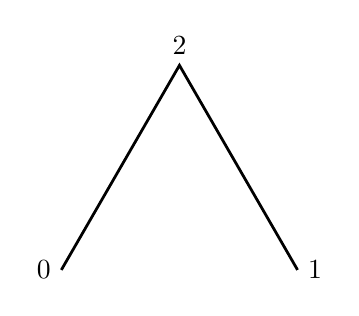
\begin{tikzpicture}
			 \draw [line width=1pt] (0,0) node[left] {$0$} -- (60:3) node[above] {$2$}  
			-- (3,0) node[right] {$1$}  ;
		\end{tikzpicture}
		\end{center}
	i.e., \[X_-=C(0),\text{ $X_+=$ cone on $S^0=\{\{0\},\{1\}\}$}\]
	$X_+\cap X_-=S^0$. Use the Mayer-Vietoris Theorem, so,
	\[H_1(X_+)\oplus H_1(X_-)\rightarrow H_1(S^1)\rightarrow H_0(S^0)
	\rightarrow H_0(X_+)\oplus H_0(X_-)\rightarrow H_0(S^1)\]
	\[0\rightarrow H_1(S)\rightarrow \mathbb{F}\oplus\mathbb{F}
	\rightarrow \mathbb{F}\oplus\mathbb{F}\rightarrow \mathbb{F}\]
	$\dim(H_1(S^1))=1$ follows from Whitehead's lemma.
\end{proof}

\begin{lemma}
	Let \[0\rightarrow V_n\xrightarrow{f_n} V_{n-1}\xrightarrow{f_{n-1}}
	\ldots\rightarrow
	V_1\xrightarrow{f_1} V_0\rightarrow 0\] be an exact sequence of finite
	dimensional vector spaces. Then,
	\[\sum_{n\geq0}\dim(V_{2n})=\sum_{n\geq0}\dim(V_{2n+1})\]
\end{lemma}

\begin{proof}
	Let $P(n)$ denote the induction hypothesis on $n$.
	\[0\rightarrow V_1\rightarrow V_0\rightarrow 0\]
	then $P(1)$ holds. The sequence is exact which implies $V_1\cong V_0$.
	Now suppose we have an exact sequence,
	\[0\rightarrow V_2\xrightarrow{f_2}V_1\xrightarrow{f_1}V_0\rightarrow 0\]
	then by the kernel-rank theorem, this implies that
	\[\dim(V_0)+\dim(V_2)=\dim(V_1)\] and so $P(2)$ is true. Now we prove
	that $P(2n)\implies P(2n+1)$. Suppose that $P(2n)$ is true, and take
	the following exact sequence,
	\[0\rightarrow V_{2n+1}\xrightarrow{f_{2n+1}}V_{2n}\xrightarrow{f_{2n}}
	V_{2n-1}\rightarrow\ldots\rightarrow V_0\rightarrow 0\] Split the sequence and define $f=\text{im}(f_{2n})=\ker(f_{2n-1})$. Now we have two exact sequences,
	\[0\rightarrow V_{2n+1}\rightarrow V_{2n}\rightarrow f\rightarrow 0\]
	and \[0\rightarrow f\rightarrow V_{2n-1}\rightarrow\ldots\rightarrow V_0
	\rightarrow 0\] By $P(2n)$, \[\dim(f)+\sum_{r=0}^{n-1}\dim(V_{2r})=
	\sum_{r=0}^{n-1}\dim(V_{2r+1})\] and $\dim(f)=\dim(V_{2n})-\dim(V_{2n+1})$.
	Substitute this into the previous expression and we get,
	\[\sum_{r=0}^n\dim(V_{2r})-\dim(V_{2n+1})=\sum_{r=0}^{n-1}\dim(V_{2r+1})\]
	This proves that $P(2n)\implies P(2n+1)$. To prove that
	$P(2n+1)\implies P(2n+2)$, take
	\[0\rightarrow V_{2n+2}\rightarrow V_{2n+1}\rightarrow
	V_{2n}\rightarrow\ldots\] Split the exact sequence as before and
	proceed as before. (Set $f=\text{im}(f_{2n+1})=\ker(f_{2n})$)
\end{proof}

\begin{lemma}{(Five lemma)}
	Suppose we have a commutative diagram of abelian groups and homomorphisms,
	\[
	\begin{tikzcd}
		A_0\arrow{r}{\alpha_0} \arrow{d}{f_0} & A_1 \arrow{r}{\alpha_1}
		\arrow{d}{f_1} & A_2 \arrow{r}{\alpha_2} \arrow{d}{f_2} &
		A_3 \arrow{r}{\alpha_3} \arrow{d}{f_3} & A_4 \arrow{d}{f_4} \\
		B_0 \arrow{r}{\beta_0} & B_1 \arrow{r}{\beta_1} & B_2 \arrow{r}{\beta_2}
		& B_3 \arrow{r}{\beta_3} & B_4
	\end{tikzcd}
	\]
	in which both rows are exact, and $f_0, \,f_1, \,f_3, f_4$ are
	isomorphisms. Then $f_2$ is also an isomorphism.
\end{lemma}

\begin{proof}
	We first show that $f_2$ is injective. Suppose $x\in A_2$ such
	that $f_2(x)=0$. We want to show that $x=0$.
	\[\beta_2 f_2(x)=0\implies f_3\alpha_2(x)=0\]
	but $f_3$ is an isomorphism, which implies that $\alpha_2(x)=0$.
	But then $x\in\ker(\alpha_2)=\text{im}(\alpha_2)$, so $x=\alpha_1(y)$
	for some $y\in A_1$. \[f_2\alpha_1(y)=0\implies \beta_1 f_1(y)=0\]
	so $f_1(y)\in\ker(\beta_1)=\text{im}(\beta_0)$.
	Thus there exists $w\in\beta_0$
	such that $\alpha_0(w)=f_1(y)$. But $f_0$ is surjective so write
	\[w=f_0(z), \,\alpha_0 f_0(z)=f(y)\implies f_1\alpha_0(z)=f_1(y)\]
	but now $f_1$ is an isomorphism so $y=\alpha_0(z), \,x=\alpha_1(y)=
	\alpha_1\alpha_0(z)$. By exactness, $\alpha_1\alpha_0=0$, so $\alpha=0$

	\vspace{12pt}

	Now we show that $f_2$ is surjective. Take $b\in\beta_2$. We want to find
	$a\in A_2$ such that $f_2(a)=b$. Now, $\beta_2(b)\in B_3$. $f_2$ is an 
	isomorphism so choose $x\in A_3$ so that \[f_3(x)=\beta_2(b)
	\implies \beta_3 f_3(x)=\beta_3\beta_2(b)\] However by exactness,
	$\beta_3\beta_2=0$, so $\beta_3f_3(x)=0\implies f_4\alpha_3(x)=0$.
	Now $f_4$ is an isomorphism thus $\alpha_3(x)=0$, $x\in\ker(\alpha_3)
	=\ker(\alpha_2)$. Now there exists $y\in A_2$ such that $\alpha_2(y)=x$.
	Consider $b-f_2(y)$. Then \[\beta_2(b-f_2(y))=\beta_2(b)-\beta_2f_2(y)
	=\beta_2(b)-f_3\alpha_2(y)=\beta_2(b)-f_3(x)=0\] Thus
	$b-f_2(y)\in\ker(\beta_2)=\ker(\beta_1)$ so there exists $w\in\beta_1$
	such that $\beta_1(w)=b-f_2(y)$. $f_1$ is an isomorphism implies that
	there exists $z\in A_1$ such that $f_1(z)=w$. So \[\beta_1f_1(z)=b-f_2(y)\]
	\[f_2\alpha_1(z)=b-f_2(y)\implies b=f_2(y+\alpha_1(z))\]
	Let $a=y+\alpha_1(z)$ which implies $b=f_2(a)$. Thus $f_2$ is surjective.
\end{proof}

\section{Subdivision}
We will now show that homology is invariant under 'subdivision'. We first have to illustrate
what 'subdivision' means. \\

Take for example $\Delta^2$ (the triangle), and add a point at its barycenter,
adding edges from the barycenter to each three of the vertices of $\Delta^2$.
We end up with an additional point (vertex), two additional regions and three additional
edges. This is an example of an easy subdivision.

\begin{definition}
	Let $X=(V_X,\mathcal{S}_X)$ be a finite simplicial complex, and let $\tau\in\mathcal{S}_X$.
	$\hat{\tau}$ will denote the subcomplex of $X$ determined by $\tau$.
	\[V_{\hat{\tau}}=\tau, \,\,\,\mathcal{S}_{\hat{\tau}}=\{p\in\mathcal{S}_X, \,p\subset\tau\}\]
	We say that $\sigma\in\mathcal{S}_X$ is \emph{principal} (or maximal) when $\sigma$ is not
	contained properly in any other simplex.
\end{definition}

\begin{proposition}
	If $\sigma_1,\ldots,\sigma_N$ are the principal simplices of $X$ then 
	\[X=\hat{\sigma_1}\cup\hat{\sigma_2}\cup\ldots\cup\hat{\sigma_N}\]
\end{proposition}

\subsection{Subdivision at a principal simplex}
Let $\sigma$ be a principal simplex of $X$ and let $\sigma_1,\ldots\sigma_N$ be the remaining
principal simplices such that \[X=\hat{\sigma}\cup\hat{\sigma_1}\cup\ldots\cup\hat{\sigma_N}\]
Put $X_+=\hat{\sigma}$, $X_-=\hat{\sigma_1}\cup\ldots\cup\hat{\sigma_N}$. Then 
$X=X_+\cup X_-$ and $X_+\cap X_-\subset\partial\hat{\sigma}$ (boundary of $\hat{\sigma}$)

\begin{definition}
	\[Sd(X,\sigma)=C(\partial\sigma)\cup\hat{\sigma_1}\cup\ldots\cup\hat{\sigma_N}\] i.e.,
	\[Sd(X\sigma)=X_+'\cup X_-'\] where $X_+'$ is the cone on the boundary of $\sigma$ and
	\[X_-'=X_-=\hat{\sigma_1}\cup\ldots\cup\hat{\sigma_N}\] and \[X_+'\cap X_-'=X_+\cap X_-\]
\end{definition}

Taking our $\Delta^2$ example earlier, letting $\sigma=\Delta^2$, $Sd(\Delta^2,\sigma)$ is 
exactly the resulting simplex we get by performing our subdivision earlier.

\subsection{Squash mapping}
Let $\sigma$ be an $n$-simplex and consider $C(\partial\sigma)$. We construct simplicial mappings
$C(\partial\sigma)\rightarrow\sigma$ as follows,
\[Sq|_{\partial\sigma}=\text{id}_{\partial\sigma}\] \[Sq(*)=\text{some (arbitrarily chosen)
vertex in }\partial\sigma\] where $*$ is our cone point.

\begin{proposition}
	$Sq:H_k(C(\partial\sigma))\rightarrow H_k(\sigma)$ is an isomorphism for all $k$.
\end{proposition}

\begin{proof}
	$C(\partial\sigma)$ and $\sigma$ are both cones, so $H_k(C(\partial\sigma))=H_k(\sigma)=0$ if 
	$k>0$. For $k=0$, any vertex $V$ in $C(\partial\sigma)$ gives a basis $[v]$ for 
	$H_0(C(\partial\sigma))$ (any two vertices differ by a boundary). Likewise, any vertex $w$
	in $\sigma$ gives basis element $[w]$ in $H_0(\sigma)$ and $Sq([v])=[w]$, so now 
	\[Sq:H_0(C(\partial\sigma))\xrightarrow{\cong}H_0(\sigma)\]
\end{proof}

\begin{theorem}
	Let $K$ be a finite complex. Let $\sigma$ be a principal complex, and let 
	$\sigma_1,\ldots,\sigma_N$ be the remaining principal simplices and define an extended
	squash map $Sq:Sd(X,\sigma)\rightarrow X$ by 
	\[Sq:C(\delta\sigma)\rightarrow\sigma\text{ is a squash mapping}\]
	\[Sq:\sigma_i\rightarrow\sigma_i\text{ identity }i=1,\ldots,N\]
	Then $Sq:H_k(Sd(X,\sigma))\rightarrow H_k(X)$ is an isomorphism for all $k$.
\end{theorem}

\begin{proof}
	Put \[X_+=\hat{\sigma}, \,X_+'=C(\partial\sigma)\]
	\[X_-'=X_-=\hat{\sigma_1}\cup\ldots\cup\hat{\sigma_N}\] so $X_+'\cap X_-'=X_+\cap X_-$ and
	$Sq:X_-'\rightarrow X_-$ is the identity. Consider the Mayer-Vietoris sequences \\
	\vspace{12pt}
	\adjustbox{scale=0.8,center}{%
		\begin{tikzcd}
			H_n(X_+'\cap X_-')\arrow{r}\arrow{d}{\text{id}} & H_n(X_+')\oplus H_n(X_-') \arrow{r}\arrow{d}{M} &
			H_n(Sd(X,\sigma) \arrow{r} \arrow{d}{Sq} & H_{n-1}(X_+'\cap X_-') \arrow{r} \arrow{d}{\text{id}} & 
			H_{n-1}(X_+')\oplus H_{n-1}(X_-') \arrow{d}{M} \\
			H_n(X_+\cap X_-) \arrow{r} & H_n(X_+)\oplus H_n(X_-) \arrow{r} & H_n(X) \arrow{r}
			& H_{n-1}(X_+\cap X_-) \arrow{r} & H_{n-1}(X_+)\oplus H_{n-1}(X_-)
		\end{tikzcd}
	} \\
	\vspace{12pt}
	where $M=\begin{pmatrix}Sq&0\\0&\text{id}\end{pmatrix}$. $\text{id}$ is clearly an
	isomorphism, as well as $M$, since $Sq:H_n(X_+')\rightarrow H_n(X_+)$ is an isomorphism.
	By the five lemma, $Sq$ is an	isomorphism.
\end{proof}

We have now shown that if $Sd(X,\sigma)$ is the subdivision of $X$ at a principal simplex,
then $H_*(Sd(X,\sigma))\cong H_*(X)$. Now we have to show that this also holds for
non-principal simplices.

\subsection{Subdivision at a non-principal simplex}
We first describe an example of a non-principal simplex. Take $\Delta^2$. Then take $\{0,1\}$.
This is contained within $\{0,1,2\}$, hence this is a non-principal simplex. We wish to 
perform subdivisions at simplices such as these.
\begin{definition}[Join]
	Let $K=(V_K,\mathcal{S}_K)$ and $L=(V_L,\mathcal{S}_L)$ be simplicial complexes such that
	$V_K\cap V_L=\emptyset$. Define 
	\[K*L=(V_K\cup V_L, \,\mathcal{S}_K\cup\mathcal{S}_L\cup\{p\cup\tau, p\in\mathcal{S}_K,\tau\in\mathcal{S}_L\}\]
	A special case is where $K=\text{point}$, so then $K*L=C(L)$.
\end{definition}

\begin{proposition}
	\[\Delta^{m+n+1}\cong\Delta^m*\Delta^n\]
\end{proposition}

\begin{proof}
	Vertex set of $\Delta^{m+n+1}$ is \[\{0,\ldots,m+n+1\}=\{0,\ldots,m\}\cup\{m+1,\ldots,m+n+1\}\] There is a 1-1 correspondence between the last set and \[0,\ldots,n\] so if we take 
	as our model of $\Delta^n$ the vertex set $\{m+1,\ldots,m+n+1\}$ and simplices to be all the
	non-empty subsets, we get $\Delta^{m+n+1}=\Delta^m*\Delta^n$ (the dimension goes up by 1).
\end{proof}

Note also that $S^m*S^n\cong S^{m+n+1}$. If $k$ is a single point $pt$, then
$C(L)=\{pt\}*L$. \\

Join is associative. If $K,L,M$ are simplicial complexes with no vertices in common, then
\[(K*L)*M\equiv K*(L*M)\]

\begin{corollary}
	If $K,L$ are disjoint complexes, then $C(K)*L\cong C(K*L)$
\end{corollary}
So the join of a cone to anything is a cone.

\subsection{Star and Link}
\begin{definition}[Star neighbourhood]
	Let $\tau$ be a simplex of $X$, and let $\sigma_1,\ldots,\sigma_N$ be the principal
	simplices which contain $\tau$. Then 
	\[St(\tau,X)=\hat{\sigma_1}\cup\ldots\cup\hat{\sigma_N}=\text{\emph{star neighbourhood} of $\tau$ 
	in $X$}\]
\end{definition}

\begin{definition}[Link]
	Let $X$ be a simplicial complex and $\rho,\tau$ be simplices of $X$ such that 
	$\rho\cap\tau=\emptyset$. We say that $\rho$ is joinable to $\tau$ in $X$ (i.e.,
	$\rho\cup\tau=p*\tau$). The \emph{link} of $\tau$ in $X$, $Lk(\tau,X)$ consists of all
	these simplices of $\rho$ of $X$ such that $\rho\cap\tau=\emptyset$ and $\rho\cap\tau$ is
	a simplex, i.e., $\rho$ is joinable to $\tau$.
\end{definition}

\begin{eg}
	star and link example
\end{eg}

\begin{proposition}
	If $\tau$ is a simplex of $X$, then $St(\tau,X)=\hat{\tau}*Lk(\tau,X)$
\end{proposition}

\begin{proof}
	The case where $\tau$ is principal is empty here. So suppose $\tau$ is not principal.
	Let $\sigma$ be a principal simplex with $\tau\subset\sigma$. Write
	\[\tau=\{v_0,\ldots,v_m\} \,\,\,m<n\] \[\sigma=\{v_0,\ldots,v_m,v_{m+1},\ldots,v_n\}\]
	Put $\rho=\{v_{m+1},\ldots,v_n\}$ so then \[\sigma=\tau*\rho\] Do this for every principal
	simplex which contains $\tau$. Each $\sigma_1=\tau*\rho_i$ for some $\rho_i$, so 
	\[\bigcup\sigma_i=\tau*(\cup\rho_i)=\tau*Lk(\tau,X)\]
\end{proof}

\begin{definition}[Subdivision at a non-principal simplex]
	Let $X$ be a finite simplicial complex, and $\tau$ a non-principal simplex.
	Let $\sigma_1,\ldots,\sigma_m$ be the principal simplices which contain $\tau$.
	Let $\sigma_{m+1},\ldots,\sigma_N$ be the remaining principal simplices.
	Put \[X_+=\hat{\sigma_1}\cup\ldots\cup\hat{\sigma_m}=St(\tau,X)\]
	\[X_-=\hat{\sigma_{m+1}}\cup\ldots\cup\hat{\sigma_N}\]
	\[X=X_++X_- \,\,\,(X_+\cap X_-\cap\tau\subset \partial\sigma)\]
	and put 
	\[X_+'=C(\partial\tau)*Lk(\tau,X)\]
	\[X_-'=X_-\] Define \[Sd(X,\tau)=X_+'\cup X_-'\] \[Sd=(C(\partial\tau)*Lk)\cup X_-'\]
	We have $Sq:C(\partial\tau)\rightarrow\tau$. Extend by identity to 
	$Sq:C(\partial\tau)*Lk\rightarrow\tau*Lk$ by identity on $Lk$. Extend again by identity
	on $X_-'=X_-$, $Sq:Sd(X,\tau)\rightarrow X$
\end{definition}

\begin{proposition}
	$Sq:Sd(X,\tau)\rightarrow X$ induces an isomorphism on homology.
\end{proposition}

\begin{proof} \[\]
	\adjustbox{scale=0.8,center}{%
		\begin{tikzcd}
			H_n(X_+'\cap X_-')\arrow{r}\arrow{d}{\text{id}} & H_n(X_+')\oplus H_n(X_-') \arrow{r}\arrow{d}{M} &
			H_n(Sd(X,\tau) \arrow{r} \arrow{d}{Sq} & H_{n-1}(X_+'\cap X_-') \arrow{r} \arrow{d}{\text{id}} & 
			H_{n-1}(X_+')\oplus H_{n-1}(X_-') \arrow{d}{M} \\
			H_n(X_+\cap X_-) \arrow{r} & H_n(X_+)\oplus H_n(X_-) \arrow{r} & H_n(X) \arrow{r}
			& H_{n-1}(X_+\cap X_-) \arrow{r} & H_{n-1}(X_+)\oplus H_{n-1}(X_-)
		\end{tikzcd}
	} \\
	\vspace{12pt}
	where $M=\begin{pmatrix}Sq&0\\0&\text{id}\end{pmatrix}$. Apply the five lemma to show 
	$Sq$ induces an isomorphism.
\end{proof}
So now we've proved the following,

\begin{theorem}
	Homology is invariant under subdivision.
\end{theorem}

\begin{eg}
	subdivision isomorphism example
\end{eg}

We now have a functor $H_n$ which takes simplicial complexes to vector spaces, and 
simplicial maps to linear maps, e.g.,
if 
\[\begin{tikzcd}
	X\ar[r,"f"]\ar[rr,out=-30,in=210,swap,"g\circ f"] & Y\ar[r,"g"] & Z
	\end{tikzcd}\]
then
\[\begin{tikzcd}
	H_n(X)\ar[r,"H_n(f)"]\ar[rr,out=-30,in=210,swap,"H_n(g\circ f)"] & H_n(Y)\ar[r,"H_n(g)"] & 
	H_n(Z)
	\end{tikzcd}\]

\noindent\underline{Properties of functors:}
\begin{enumerate}
	\item $H_n(g\circ f)=H_n(g)\circ H_n(f)$
	\item $H_n(\text{id})=\text{id}_{H_n}$ i.e., \[\text{id}:X\rightarrow X, \,
	H_n(\text{id}):H_n(X)\rightarrow H_n(X)\]
\end{enumerate}

As a consequence, if $f:X\rightarrow Y$ is an isomorphism, then
$H_n(f):H_n(X)\rightarrow H_n(Y)$ is an isomorphism.

\begin{proof}
	If $g=f^{-1}:Y\rightarrow X$, $g\circ f=\text{id}_X, \,f\circ g=\text{id}_Y$ then
	\[H_n(g)\circ H_n(f)=\text{id}, \,H_n(f)\circ H_n(g)=\text{id}\] so
	\[H_n(g)=H_n(f)^{-1}\]
\end{proof}

But we have established a stronger property, that is, $H_n$ is invariant under subdivision,
i.e., if $Y$ subdivides $X$, then $H_n(Y)\cong H_n(X)$.

\begin{definition}
	Let $X,Y$ be simplicial complexes. We say that $X,Y$ are \emph{combinatorially equivalent}
	(written $X\sim Y$) if and only if there exists a finite sequence $(X_r)_{0\leq r\leq N}$ of
	complexes $X_r$ such that $X_0=X, \,X_N=Y$ and for each $r, \,0\leq r\leq N-1$, either
	$X_{r+1}$ is a subdivision of $X_r$ or $X_r$ is a subdivision of $X_{r+1}$.
\end{definition}

\begin{corollary}
	If $X\sim Y$ then $H_n(X)\cong H_n(Y)$.
\end{corollary}

\noindent So we won't worry too much about how we triangulate things.

\vspace{12pt}

Consider $S^2=\Delta^3\text {with the interior missing}$. This is the minimal model
of $S^2$. The dodecahedron is also a model of $S^2$ obtained from the minimal model
by a sequece of subdivisions, hence for any model of $S^2$,
\[H_k(S^2,\mathbb{F})
	\begin{cases}
		\mathbb{F}&k=0\\0&k=1\\\mathbb{F}&k=2\\0&k>2
	\end{cases}\] 

We note that the usual definition of $S^2$ is given by 
\[S^2=\{\begin{pmatrix}x_1\\x_2\\x_3\end{pmatrix}\in\mathbb{R}^3\,:\,
x_1^2+x_2^2+x_3^2=1\}\] Now we define $S^1(n)$ to be the model of the circle $S^1$ with
$n$-subdivision points ($n\geq3$), so \[S^1(n)\sim S^1(m)\,\,\,\forall m,n\geq3\]

so for example, $S^1(3)$ is the triangle, $S^1(4)$ is the square, $S^1(5)$ the pentagon, and so on.

\section{Orientation Theorem}
\begin{definition}[Orientability]
	We say that a surface $\Sigma$ is orientable if and only if it is possible to orient
	each $2$-simplex in such a way that every $1$-simplex receives the opposite orientations
	from its containing $2$-simplices.
\end{definition}

\begin{eg}
	orientability of $T^2$
\end{eg}

\subsection{{Euler characteristic}}
\begin{definition}
	Let $X=(V_X,\mathcal{S}_X)$ be a finite simplicial complex. Let $c_n$ be the number of
	$n$-simplices of $X$, \[c_n(X)=c_n=\text{no. of $n$-simplices of $X$}\] we define
	\[\chi_\text{geom}(X)=\sum_{n}(-1)^n c_n(X)\]
	This is known as the \emph{geometric} Euler characteristic. \\

	Put $h_n^\mathbb{F}(X) = \dim H_n(X;\mathbb{F}) (=h_n)$, and define
	\[\chi_\text{hom}^\mathbb{F}(X)=\sum_n (-1)^n h_n^\mathbb{F}(X)\]
	This is known as the \emph{homological} Euler characteristic.
\end{definition}

We will show that 
\begin{theorem}
	\[\chi_\text{hom}^\mathbb{F}(X)=\chi_\text{geom}(X)\]
\end{theorem}
In particular $\chi_\text{hom}^\mathbb{F}$ is independent of $\mathbb{F}$, so we'll ignore
$\mathbb{F}$.

\begin{proof}
	Fix a field $\mathbb{F}$. $c_n=c_n(X)=\text{no. of $n$-simplices of $X$}$
	\[c_n=\dim C_n(X;\mathbb{F})\] so put $h_n=\dim H_n(X;\mathbb{F})$ and look at the 
	sequence
	\[C_{n+1}(X)\xrightarrow{\partial_{n+1}}C_n(X)\xrightarrow{\partial_n}C_{n-1}(X)\]
	\[H_n(X)=\ker\partial_n/\text{im}\partial_{n+1}=Z_n(X)/B_n(X)\]
	Put $z_n=\dim\ker\partial_n, \,b_n=\dim\text{im}(\partial_{n+1})$ so 
	\[z_n=h_n+b_n\] However by the kernel-rank theorem,
	\[c_n=z_n+b_{n-1}\] hence \[c_n=h_n+b_n+b_{n-1}\]
	Now take the alternating sum 
	\[\sum_{n} (-1)^n c_n=\sum_n (-1)^n h_n +\sum_n (-1)^n (b_n+b_{n-1})\]
	The last term on the RHS evaluates to 0, and recognising what the other two sums are, we
	have \[\chi_\text{hom}^\mathbb{F}(X)=\chi_\text{geom}(X)\]
\end{proof}

As $H_*(X;\mathbb{F})$ is invariant under subdivision, it follows that $\chi_\text{geom}(X)$
is the same as well, so from now on, we will usually just write $\chi(X)$.

\begin{eg}
	euler characteristic examples
	homology of real projective plane example
\end{eg}

\begin{definition}[Connected sum of surfaces]
	Let $\Sigma, \,\Sigma'$ be surfaces. Let $\sigma$ be a $2$-simplex in $\Sigma, \,\sigma'$ 
	be a $2$-simplex in $\Sigma'$. Let $\Sigma_0$ be the complex obtained from $\Sigma$ by 
	removing $\sigma$. Likewise for $\Sigma_0'$. Formally,
	\[\Sigma\#\Sigma'=\Sigma_0\bigcup_{\partial=\partial'}\Sigma_0'\]
	(i.e., we glue the boundaries of $\Sigma_0$ and $\Sigma_0'$ together.)
\end{definition}

\begin{proposition}
	\[\chi(\Sigma\#\Sigma')=\chi(\Sigma)+\chi(\Sigma')-2\]
\end{proposition}

\begin{eg}
	examples of orientable surfaces, 2-sphere, 2-torus, etc.
\end{eg}

\begin{theorem}[Classification Theorem for Surfaces]
	placeholder
\end{theorem}

Recall that if $\sigma$ is a simplex of $X$, then $Lk(\sigma, X)$ is equal to the complex where simplices $\tau$ satisfy $\sigma\cap\tau=\emptyset$, where $\sigma\cup\tau$ is a simplex
of $X$. \\

A simplicial surface $\Sigma$ is a complex in which \[Lk(v,\Sigma)\cong S^1(N)\] where
$v$ is a vertex of $\Sigma$ ($N\geq3$). Recall that $S^1(N)$ is the circle with $N$ 
subdivision points, for example, $S^1(5)$ is 'the' pentagon. \\

Observe that in $S^1(N)$, every vertex belongs to exactly \emph{two} 1-simplices.

\begin{proposition}
	If $\Sigma$ is a simplicial surface then every 1-simplex lies in exactly two 2-simplices.
\end{proposition}

\begin{proof}
	Let $\rho=[v_0, v_1]$ be a 1-simplex. $Lk(v_0,\Sigma)\cong S^1(N)$, $v_1\in Lk(v_0,\Sigma)$
	and $v_1$ belongs to exactly two 1-simplices, say $\tau_0,\tau_1$, so then
	\[\tau_0*\{v_0\},\,\tau_1*\{v_0\}\] are the two 2-simplices which contain $\rho$.
\end{proof}


\subsection{Copath}
\begin{definition}
	Let $X$ be a simplicial complex of dimension 2. Let $\sigma,\sigma'$ be 2-simplices in 
	$X$. A \emph{copath} from $\sigma$ to $\sigma'$ is a collection of 2-simplices
	\[\{\sigma_0,\sigma_1,\ldots,\sigma_N\}\] such that $\sigma_0=\sigma,\,\sigma_N=\sigma'$
	and $\sigma_r\cap\sigma_{r+1}$ is a 1-simplex for $0\leq r\leq N-1$.
\end{definition}

\begin{theorem}
	If $\Sigma$ is a connected simplicial surface and $\sigma,\sigma', \,\sigma\neq\sigma'$ are 2-simplices in $\Sigma$ then there exists a copath $(\sigma_0,\ldots,\sigma_N)$ from 
	$\sigma$ to $\sigma'$.
\end{theorem}

\begin{proof}
	Consider $\sigma\cap\sigma'$. A priori we have 4 cases
	\begin{enumerate}
		\item $|\sigma\cap\sigma'|=3$. This is impossible, as this implies $\sigma=\sigma'$
		\item $|\sigma\cap\sigma'|=2$. Put $\rho=\sigma\cap\sigma'$ which is a 1-simplex, where
					$\rho$ lies in exactly two 2-simplices which are $\sigma,\sigma'$ and now 
					$(\sigma,\sigma')$ is a copath from $\sigma$ to $\sigma'$
		\item $|\sigma\cap\sigma'|=1$. $\sigma\cap\sigma'=\{v\}$ for some vertex $v$. Look at 
					$Lk(v,\Sigma)$. Write \[\sigma=\{v,u,u_0\}\]\[\sigma'=\{v,w,w_0\}\] We know 
				$v,w\in Lk(v,\Sigma)\cong S^1(N)$ which is connected. So choose a path in 
				$Lk(v,\Sigma)$ from $u$ to $w$ \[\xi=(\xi_0,\ldots,\xi_N)\]\[\xi_0=u,\ldots,\xi_N=w\]
				Then $[\xi_i,\xi_{i+1}]$ is a 1-simplex in $Lk(v,\Sigma)$. Define 
				$\sigma_i=\{v,\xi_i,\xi_{i+1}\}$ which is a 2-simplex, and then we have 
				that $\sigma_0,\ldots,\sigma_N$ is a copath from $\sigma$ to $\sigma'$.
		\item $\sigma\cap\sigma'=\emptyset$. Let $N$ be a shortest path from a vertex $v$ of 
				$\sigma$ to a vertex $v'$ of $\sigma'$. We proceed by induction on $N$. The induction
				base case here is when $N=1$. $(v,v')$ sits inside two 2-simplices. Choose one of 
				them and call it $\tau$. $\sigma\cap\tau=\{v\}$ so there exists a copath from 
				$\sigma$ to $\tau$. Similarly, $\sigma'\cap\tau=\{v'\}$ so there exists a copath 
				from $\tau$ to $\sigma'$. Compare the two copaths to get a copath from $\sigma$ 
				to $\sigma'$. \\

				Now for our induction step (assume hypothesis proved for $N-1$), let 
				$v\in\sigma, \,v'\in\sigma'$. Let $(w_0,\ldots,w_M)$ be a shortest path from 
				$v$ to $v'$. Let $\tau$ be any 2-simplex such that $w_{m-1}\in\tau$. By 
				our induction hypothesis, there exists a copath from $\sigma$ to $\tau$. By 
				the induction base, there exists a copath from $\tau$ to $\sigma'$. Compose the 
				two copaths to get a copath from $\sigma$ to $\sigma'$.
	\end{enumerate}
\end{proof}

\subsection{Orientation Theorem}
\begin{theorem}[Orientation Theorem]
	Let $\Sigma$ be a connected simplicial surface, and let $\mathbb{F}$ be a field.
	\begin{enumerate}
		\item If $1+1\neq0$ in $\mathbb{F}$ and $\Sigma$ is orientable then
		\[H_2(\Sigma;\mathbb{F})\cong\mathbb{F}\]
		\item If $1+1\neq0$ in $\mathbb{F}$ and $\Sigma$ is non-orientable then 
		\[H_2(\Sigma;\mathbb{F})=0\]
		\item If $1+1=0$ then \[H_2(\Sigma;\mathbb{F})\cong\mathbb{F}\] regardless if $\Sigma$
		is orientable or not.
	\end{enumerate}
\end{theorem}

\begin{definition}[Intersection number]
	\[\langle[v_0,v_1,v_2],[v_0,v_1]\rangle=+1\]
	\[\partial[v_0,v_1,v_2]=[v_1,v_2]-[v_0,v_2]+[v_0,v_1]\]
	\[\langle[v_0,v_1,v_2],[v_0,v_2]\rangle=-1\]
	\[\langle[v_0,v_1,v_2],[v_1,v_2]\rangle=+1\]

	\noindent More generally,
	\[\langle[v_{\sigma(0)},v_{\sigma(1)},v_{\sigma(2)}],[v_0,v_1]\rangle=sgn(\sigma)\]
	\[\langle[v_{\sigma(0)},v_{\sigma(1)},v_{\sigma(2)}],[v_0,v_2]\rangle=-sgn(\sigma)\]
	\[\langle[v_{\sigma(0)},v_{\sigma(1)},v_{\sigma(2)}],[v_1,v_2]\rangle=sgn(\sigma)\]
\end{definition}

\begin{proof}[(of Orientation Theorem)]
	For each 1-simplex $\rho$ of $\Sigma$, fix once and for all a specific orientation 
	$\hat{\rho}$ of $\rho$. \\

	Let $\Sigma_1,\ldots,\Sigma_N$ be a list of the 2-simplices of $\Sigma_1,\ldots,\Sigma_N$
	be a list of the 2-simplices of $\Sigma$ and $\hat{\Sigma_i}$ fixed orientation of
	$\Sigma_i$. To change the orientations on 2-simplices, we need a function 
	\[\eta:\{1,\ldots,N\}\rightarrow\{\pm1\}\]
	$\eta(i)\hat{\sigma_i}$ is the oriented 2-simplex which is 
	\[\begin{cases}
		\hat{\sigma_i}&\eta(i)=1 \\ \text{opposite orientation of }\hat{\sigma_i}&\eta(i)=-1
	\end{cases}\]

We shall consider elements of $C_2(\Sigma;\mathbb{F})$ of the form 
\[[\eta]=\sum_{i=1}^N\eta(i)\hat{\sigma_i}\in C_2(\Sigma;\mathbb{F})\] We want to calculate 
$\partial[\eta]$. \\

Fix a 1-simplex $\rho$ and let $\sigma_s,\sigma_t$ be the adjacent 2-simplices which contain 
$\rho$. The coefficient of $\hat{\rho}$ in $\partial[\eta]$ is simply
\[[\eta(s)\hat{\sigma_s},\hat{\rho}]+[\eta(t)\hat{\sigma_t},\hat{rho}]=\begin{cases}
	2\\0\\-2
\end{cases}\]
To ensure that $\partial[\eta]=0$ we require $\eta$ to satisfy 
\[[\eta(s)\hat{\sigma_s},\hat{\rho}]+[\eta(t)\hat{\sigma_t},\hat{rho}]=0\]
i.e.,
\[\langle\eta(s)\hat{\sigma_s,p}\rangle+\langle\eta(t)\hat{\sigma_t,\hat{rho}}\rangle=0\,\,\,(*)\]
whenever $\sigma_s,\sigma_t$ are adjacent, and now we know
$\Sigma$ is orientable if and only if there exists a function \[\eta:\{1,\ldots,N\}
\rightarrow\{\pm1\}\] such that we have $(*)$ whenever $\sigma_s,\sigma_t$ are adjacent. \\

So when $\Sigma$ is orientable and $\eta:\{1,\ldots,N\}\rightarrow\{\pm1\}$ is an orientation,
then $[\eta]\in Z_2(\Sigma)$ and so defines a non-zero element of $H_2(\Sigma;\mathbb{F})$. \\

Now we show that when $\Sigma$ is orientable, \[H_2(\Sigma;\mathbb{F})\cong\mathbb{F}\] and
$[\eta]$ is a \emph{generator}. \\

Let us consider the elements 
\[\sum_{s=1}^N a_s\hat{\sigma}_s\in C_2(\Sigma;\mathbb{F})\] where $a_s\in\mathbb{F}$.
Suppose that $\rho$ is a 1-simplex and $\sigma_s,\sigma_t$ are adjacent 2-simplices which contain $\rho$. \\

We calculate $\partial(\sum a_s\sigma_s)$. The coefficients of $\hat{rho}$ is simply 
$a_s\langle\hat{\sigma_t},\hat{\rho}\rangle + a_t\langle\hat{\sigma_t},\hat{\rho}\rangle$.
If we want $\partial(\Sigma a_s\sigma_s)=0$ then 
\[a_s\langle\hat{\sigma_t},\hat{\rho}\rangle + a_t\langle\hat{\sigma_t},\hat{\rho}\rangle=0\]
for adjacent $s,t$. \[\pm a_s\pm a_t=0\] so $a_t=\pm a_s$ if $\sigma_s,\sigma_t$ are adjacent.
So going along a copath, coefficients $a_s$ are constant up to sign. \\

Fix a "base 2-simplex" $\sigma_0$ and suppose \[\partial(\sum a_s\hat{\sigma_s})=0\] Then 
going along a copath from $\sigma_0$ to $\sigma_s$, we find that $a_s=\pm a_0$. Define 
$\eta:\{1,\ldots,N\}\rightarrow\{\pm1\}$ by 
\[\eta(s)=\begin{cases}
	+1& a_s=a_0 \\ -1& a_s=-a_0
\end{cases}\]
then $\alpha=a_0[\eta]$ if $\partial\alpha=0$ which shows that $\dim H_2(\Sigma;\mathbb{F})\leq1$. \\

If $\Sigma $ is orientable, there exists global orientation $\eta:\{1,\ldots,N\}\rightarrow
\{\pm 1\}$ and $[\eta]$ generates $H_2(\Sigma;\mathbb{F})$ \\

If $\Sigma$ is non-orientable, $\partial[\eta]\neq0$ for any such $\eta$ and if 
$\alpha\in Z_2(\Sigma;\mathbb{F})$, $\alpha=\sum a_s\hat{\sigma_s}$, \[\alpha=a_o0[\eta]
\,\,\,\partial(\alpha)=a_0\partial[\eta]\]

\[\partial(\alpha)=0\implies a_0\partial[\eta]=0\] but $\partial[\eta]\neq0$ and $\alpha=0$,
so $a_0=0$, so then \[H_2(\Sigma;\mathbb{F})\] However if $1+1=0$, then 
\[\partial(\sum_{s=1}^N \hat{\sigma_s})=0\] as $\pm 2=0$ and $H_2(\Sigma;\mathbb{F})\cong
\mathbb{F}$.
\end{proof}

For surfaces, $H_0$ tells us whether the surface is connected or not. $H_2$ tells us
whether the surface is orientable or not. $H_1$ in a sense tells us how 'big' the surface is.

\newpage

\setlength{\columnsep}{-2.5cm}
    \begin{multicols}{2}
			\begin{center}
				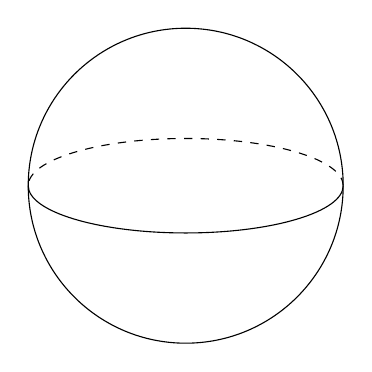
\begin{tikzpicture}
					\shade[ball color = white!40, opacity = 0.0] (0,0) circle (2cm);
					\draw (0,0) circle (2cm);
					\draw (-2,0) arc (180:360:2 and 0.6);
					\draw[dashed] (2,0) arc (0:180:2 and 0.6);
				\end{tikzpicture}
			\end{center}

			\[\Sigma_0^+, S^2, \text{  genus}=0\] \vspace{12pt}
			\[H_k=\begin{cases}\mathbb{F}&k=0\\0&k=1\\\mathbb{F}&k=2\end{cases}\]

        \vfill\null\columnbreak  % This whole line is needed to insert a column break

				\begin{center}
					\scalebox{1.75}{
					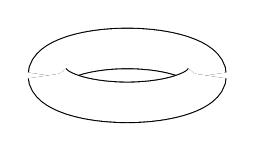
\begin{tikzpicture}[yscale=cos(70)]
						\draw[double distance=5mm] (0:1) arc (0:180:1);
						\draw[double distance=5mm] (180:1) arc (180:360:1);
					\end{tikzpicture}
					}
				\end{center}
		
				\[\Sigma_1^+, T^2, \text{  genus}=1\]
				\[H_k=
				\begin{cases}\mathbb{F}&k=0\\\mathbb{F}\oplus\mathbb{F}&k=1\\\mathbb{F}&k=2
				\end{cases}\]
    \end{multicols}

In general for $\Sigma_g^+=\text{$n$-fold torus}$, we have 
\[H_k\begin{cases}
	\mathbb{F}&k=0\\
	H_1=\mathbb{F}\oplus\ldots\oplus\mathbb{F}\,\,(2g\text{ times})&k=1\\
	\mathbb{F}&k=2
\end{cases}\]

We also have
\[\Sigma_0^-=\mathbb{R}P(2), \,\Sigma_g^-=\mathbb{R}P(2)\#\ldots\#\mathbb{R}P(2) \text{
	   ($g+1$ times)
}\]

\noindent If $1+1\neq0$, then 
\[H_k=\begin{cases}
	\mathbb{F}&k=0\\
	\mathbb{F}^g&k=1\\
	0&k=2
\end{cases}
\]

\noindent but if $1+1=0$,
\[H_k=\begin{cases}
	\mathbb{F}&k=0\\
	\mathbb{F}^{g+1}&k=1\\
	\mathbb{F}&k=2
\end{cases}
\]

\noindent As $H_*(-;\mathbb{F})$ is invariant under combinatorial equivalence ($\sim$),
we have 

\[\Sigma_g^+\sim\Sigma_h^+\implies g=h\]
\[\Sigma_g^-\sim\Sigma_h^-\implies g=h\]
\[\Sigma_g^+\not\sim\Sigma_h^-\text{ for any $g,h$}\]

\section{Some linear algebra}
\begin{proposition}
	If $A,B$ are $n\times n$ matrices over $\mathbb{F}$, then 
	\[Tr(AB)=Tr(BA)\]
\end{proposition}

\begin{proof}
	First write $A=(a_{kj}), \,B=(b_{ji})$. Then,
	\[(AB)_{ki}=\sum_{j=1}^n a_{kj}b_{ji}\]\[(AB)_{kk}=\sum_j a_{kj}b_{jk}\]
	\begin{eqnarray*}
		Tr(AB)&=&\sum_{k=1}^n\sum_{j=1}^n a_{kj}b_{jk} \\
		&=&\sum_{j=1}^n\sum_{k=1}^n a_{kj}b_{jk}
	\end{eqnarray*}
	and we know \[a_{kj}b_{jk}=b_{jk}a_{kj}\] as $\mathbb{F}$ is a field, so now 
	we have 
	\[=\sum_{j=1}^n\sum_{k=1}^n b_{jk}a_{jk}=Tr(BA)\]
\end{proof}

\begin{remark}
	Note that in general $Tr(AB)\neq Tr(A)Tr(B)$. For example, take 
	\[A=\begin{pmatrix}
		0&1\\1&0=B
	\end{pmatrix}\] so that \[AB=\begin{pmatrix}
		1&0\\0&1
	\end{pmatrix}\] and \[Tr(A)=Tr(B)=0,\,\,\,Tr(AB)=2\]
\end{remark}

\begin{corollary}
	If $A,P$ are $n\times n$ matrices over $\mathbb{F}$ and $P$ is invertible then 
	\[Tr(PAP^{-1})=Tr(A)\]
\end{corollary}

\begin{proof}
	\[Tr((PA)P^{-1})=Tr(P^{-1}PA)=Tr(A)\]
\end{proof}

\subsection{Trace of a linear map}
Let $V$ be a finite dimensional vector space over $\mathbb{F}$. Let $X:V\rightarrow V$
be a linear map. Take a basis $\{e_1,\ldots,e_n\}$ for $V$, and write 
\[X(e_i)=\sum_{j=1}^n e_j\xi_{ji}\]\[X\sim(\xi_{ji})=\xi\] We would like to define 
$Tr(X)=Tr(\xi)=\sum_{j=1}^n \xi_{ji}$ \\

However, $\xi$ depends on the choice of basis $\{e_1,\ldots,e_n\}$. Suppose we take 
another basis $\{f_1,\ldots,f_n\}$ so that $X(f_i)=\sum_{j=1}^n f_i\eta_{ji}$, \[X\sim(\eta)\]
$\eta,\xi$ are related by $\eta=P\xi P^{-1}$ where $P$ is the change of basis matrix, 
\[P=M(\text{id})_\xi^\eta,\,\,\,P^{-1}=M(\text{id})_\eta^\xi\] Consequently
\[Tr(\eta)=Tr(P\xi P^{-1})=Tr(\xi)\] so the trace is independent of the particular basis 
so we can legitimately define 
\[Tr(X)=Tr(\xi)\] when $X(e_i)=\sum_{j=1}^n e_j\xi_{ji}$.

\begin{proposition}[Additivity of $Tr$]
	Let \[0\rightarrow U\rightarrow V\xrightarrow{p}W\rightarrow 0\] be an 
	exact sequence of finite dimensional vector spaces over $\mathbb{F}$ and suppose 
	there exists linear maps $T_U,T_V,T_W$ such that the following commutes
	\[
	\begin{tikzcd}
		0\arrow{r} & U \arrow{r}
		\arrow{d}{T_U} & V \arrow{r}{p} \arrow{d}{T_V} &
		W \arrow{r}\arrow{d}{T_W} & 0\\
		0 \arrow{r}& U \arrow{r} & V\arrow{r}{p}
		& W \arrow{r} & 0
	\end{tikzcd}
	\]
	then 
	\[Tr(T_V)=Tr(T_U)+Tr(T_W)\]
\end{proposition}

\begin{lemma}
	Let $T:V\rightarrow V$ be a linear map over $\mathbb{F}$. Suppose $\dim(V)=n$, and let 
	$U\subset V$ be a subspace; $T(U)\subset U$, and $\dim(U)=k$. Then $T$ can be 
	represented by a matrix 
	\[T\sim\begin{pmatrix}
		A&B\\0&D
	\end{pmatrix}\] where $A$ is a $k\times k$ matrix, $B$ is a $k\times (n-k)$ matrix and 
	$D$ is a $(n-k)\times(n-k)$ matrix.
\end{lemma}

\begin{proof}(of lemma)
	Let $\{e_1,\ldots,e_k\}$ be a basis for $U$. Extend to a basis $\{e_1,\ldots,e_k,f_1,\ldots,f_q\}$ for $V$ ($q=n-k$). With respect to this basis, 
	\[T(e_i)=\sum_{j=1}^k e_j a_{ji}\,\,\,\,\,(T(U)\subset U)\]
	$T(f_r)$ is a linear combination in $\{e_1,\ldots,e_k,f_1,\ldots,f_q\}$. Write 
	\[T(f_r)=\sum_{s=1}^k e_s b_{sr} + \sum_{t=1}^q f_t d_{tr}\,\,\,(1\leq r\leq q)\]
	so the matrix of $T$ has block form, 
	\[T\sim\begin{pmatrix}
		A&B\\0&D
	\end{pmatrix}\] where $A=(a_{ji}), \,B=(b_{sr}), \,D=(d_{tr})$.
\end{proof}
Note that $Tr(T) = Tr(A) + Tr(D)$.

\begin{proof}(of proposition)
	Let $\{e_1,\ldots,e_k\}$ be a basis for $U$, and $\{\phi_1,\ldots,\phi_q\}$ be basis for 
	$W$. For all $r$, choose $f_r\in V, \,p(f_r)=\phi_r$. Then,
	$\{e_1,\ldots,e_k\}\cup\{f_1,\ldots,f_q\}$ is a basis for $V$. By the previous lemma, 
	$T_V$ is represented by a block matrix 
	\[T_V\sim\begin{pmatrix}
		A&B\\0&D
	\end{pmatrix}\] where $A=\text{matrix of $T_U$}$, and factoring out $U$,
	\[D=\text{matrix $T_W$ with respect to $\{f_1,\ldots,f_q\}$}\] hence 
	\begin{eqnarray*}
		Tr(T_V) &=& Tr(A) + Tr(D)\\
		&=& Tr(T_U) + Tr(T_W)
	\end{eqnarray*}
\end{proof}

\section{Lefschetz Fixed Simplex Theorem}
\begin{theorem}[Lefschetz Fixed Simplex Theorem]
	Let $f:K\rightarrow K$ be a simplicial map where $K$ is a finite simplicial complex. 
Define \[\lambda(f)=\sum_k (-1)^k Tr(H_k(f))\] If $\lambda(f)\neq0$ then there exists a 
simplex $\sigma$ of $K$ such that $f(\sigma)=\sigma$. $\lambda(f)$ is called the 
\emph{Lefschetz number} of $f$ (pick a field $\mathbb{F}$)
\end{theorem}


\begin{definition}[Geometrical Lefschetz index]
	\[\lambda_\text{geom}(f)=\sum_k (-1)^k Tr(C_k(f))\] where
	$C_k(f):C_k(K;\mathbb{F})\rightarrow C_{k-1}(K;\mathbb{F})$ is the mapping induced by $f$.
\end{definition}

\begin{definition}[Homological Lefschetz index]
	\[\lambda_\text{hom}(f)=\sum_k (-1)^k Tr(H_k(f))\]
\end{definition}

\begin{proposition}
	\[\lambda_\text{geom}(f)=\lambda_\text{hom}(f)\]
\end{proposition}

\begin{proof}
	\[
	\begin{tikzcd}
		0\arrow{r} & Z_k(K) \arrow{r}
		\arrow{d}{Z_k(f)} & C_k(K) \arrow{r} \arrow{d}{C_k(F)} &
		B_{k-1}(K) \arrow{r}\arrow{d}{B_{k-1}(f)} & 0\\
		0 \arrow{r}& Z_k(K) \arrow{r} & C_k(K) \arrow{r}
		& B_{k-1}(K) \arrow{r} & 0
	\end{tikzcd}
	\]
	\[Z_k(K)=\ker\partial_k,\,B_{k-1}(K)=\text{im}(\partial_k)\]
	so \[Tr(C_k(f)) = Tr(Z_k(K)) + Tr(B_{k-1}(K))\,\,\,(1)\]
	and we also have
	\[
	\begin{tikzcd}
		0\arrow{r} & B_k(K) \arrow{r}
		\arrow{d}{B_k(f)} & Z_k(K) \arrow{r} \arrow{d}{Z_k(F)} &
		H_{k}(K) \arrow{r}\arrow{d}{H_k(f)} & 0\\
		0 \arrow{r}& B_k(K) \arrow{r} & Z_k(K) \arrow{r}
		& H_k(K) \arrow{r} & 0
	\end{tikzcd}
	\]
	where both the rows are exact, so 
	\[Tr(Z_k(f)) = Tr(H_k(f)) + Tr(B_k(f))\,\,\,(2)\]
	Substituting $(2)$ into $(1)$, we have 
	\[Tr \,C_k(f) = Tr \,H_k(f) + Tr \,B_k(f) + Tr (B_{k-1}(f))\] but 
	\[\sum_k (-1)^k Tr \,B_k(f) + Tr \,B_{k-1}(f) = 0\]
	so 
	\[\sum_k (-1)^k Tr \,C_k(f) = \sum (-1)^k Tr \,H_k(f)\] thus 
	\[\lambda_\text{geom}(f)=\lambda_\text{hom}(f)\]
\end{proof}

\begin{remark}
	Note that $\lambda_\text{hom}(f)$ is easier to compute, but $\lambda_\text{geom}(f)$ 
	carries geometric information.
\end{remark}

Now consider $C_k(f):C_k(K)\rightarrow C_k(K)$. If $\sigma$ is a $k$-simplex of $K$, either 
$f(\sigma)$ is a $k$-simplex or $f(\sigma)$ is an $l$-simplex, where $l<k$. \\

In the first case, $C_k(f)(\sigma)$ is a basis element of $C_k$. In the second case, 
$C_k(f)(\sigma)=0$, so representing $C_k(f)$ as a matrix, in a column there is at most 
one non-zero entry. \\

List the $k$-simplices of $K$, $\sigma_1,\ldots,\sigma_N$.
$C_k(f)$ is an $N\times N$ matrix. The $(i,i)$ entry of $C_k(f)$ is non-zero if and 
only if $f(\sigma)=\pm\sigma$, so if no $k$-simplex if fixed by $f$ then the diagonal of 
$C_k(f)$ is $0$ and $Tr(C_k(f))=0$. \\

\begin{proof}[of Lefschetz fixed simplex theorem]
	Formally put, 
\[f\text{ fixes no $k$-simplex}\implies Tr \,C_k(f)=0\]
\[\text{ so $f$ fixes no simplex}\implies Tr \,C_k(f)=0\text{ for all $k$}\]
\[\text{so $f$ fixes no simplex}\implies \sum_k (-1)^k Tr \,C_k(f)=
(\lambda_\text{geom}(f)=)0\]
In the contrapositive,
\[\lambda_\text{geom}(f)\neq0\implies\text{$f$ fixes some simplex (up to sign, it may 
change local orientation)}\] hence 
\[\lambda_\text{hom}(f)\neq0\implies\text{$f$ fixes some simplex}\]
\end{proof}

Recall that 
\begin{proposition}
	If $f:K\rightarrow K$ is a simplicial map and $K$ is connected then 
	\[H_0(f)=\text{id}:H_0(K)\rightarrow H_0(K)\]
\end{proposition}

\begin{proof}
	IF $v,w$ are vertices of $K$, then $|v|-|w|\in\Im\partial_1$, so 
	$[v]=[w]$ in $H_0(K)$. Hence $[f(v)]=[v]$ in $H_0(K)$ for any vertex $v$. But any 
	vertex $v$ generates $H_0$ ($K$ connected), so 
	\[H_0(f)=\text{id}:\text{generator}\rightarrow\text{itself}\]
\end{proof}

\begin{corollary}
	If $K$ is a connected simplicial complex and $f:K\rightarrow K$ is simplicial, then 
	\[Tr \,H_0(K)=1\]
\end{corollary}

\begin{corollary}
	Let $f:K\rightarrow K$ be a simplicial map, where $K$ is a finite connected simplicial 
	complex and \[H_k(K;\mathbb{F})\text{ for }k>0\] then $\lambda(f)=1$.
\end{corollary}

\begin{corollary}
	If $f:K\rightarrow K$ is a simplicial map, $K$ a finite connected complex such that 
	$H_k(K;\mathbb{F})=0$ for $k>0$, then there exists a simplex $\sigma$ of $K$ such that 
	$f(\sigma)=\sigma$ (up to orientation.)
\end{corollary}

\begin{proof}
	\[\lambda(f)=1\neq0\]
\end{proof}

\begin{corollary}
	If $K$ is a finite simplicial complex and $K\sim CX$ (combinatorially equivalent) where 
	$CX$ is the cone on $X$, for some $X$, then any simplicial map $f:K\rightarrow K$ fixes
	a simplex.
\end{corollary}

\begin{eg}
	$K\sim \Delta^n$, any simplicial $f:K\rightarrow K$ fixes a simplex. (Brouwer Fixed Simplex)
\end{eg}

To transform a finite simplicial complex into a metric space, replace the 
formal $n$-simplex by standard geometric $n$-simplex, 
\[|\Delta^n|=\{t_0 e_0 + t_1 e_1 + \ldots + t_n e_n\,|\,t_i\geq 0, \sum_{i=0}^n t_i = 1\}\]
where $e_0, \ldots, e_n$ are the standard basis for $\mathbb{R}^{n+1}$. \\

$f:\Delta^n\rightarrow \Delta^n$ (formal simplicial mapping) gives a continuous mapping
\[|f|:|\Delta^n|\rightarrow |\Delta^n|\]
\[|f|(\sum t_i e_i)\rightarrow \sum t_i f(e_i)\] $f$ permutes $e_0, \ldots, e_n$,
\[|f|(\frac{1}{n}\sum e_i) = \frac{1}{n}\sum e_i\text{ (fixed point)}\]
so if $g:K\rightarrow K$ is a simplicial map, $K$ a finite complex, we get a continuous
mapping (!) $|g|:|K|\rightarrow |K|$. If $g$ fixes a simplex, then 
$|g|$ fixes a point.

\begin{theorem}[Brouwer Fixed Point Theorem]
	Let $X=|K|$ where $K$ is some finite simplicial complex. Suppose any simplicial map 
	$g(m):K(m)\rightarrow K(m)$ has a fixed simplex $K(m)$ (subdivision of $K$), then any 
	continuous $f:X\rightarrow X$ has a fixed point.
\end{theorem}

\begin{proof}
	Suppose $f:X\rightarrow X$ does not have a fixed point. $X$ compact, so there exists 
	$\epsilon>0$ such that $\epsilon||f(x)-x||$ for all $x$. Suppose 
	$g(m):K(m)\rightarrow K(m)$, then 
	\[||f(x)-x||\leq||f(x)-g_m(x)||+||g_m(x)-x||\] so 
	\[\forall\eta\,\,\,\exists m \,||f(x)-g_m(x)||<\eta\,\,\,\forall x\]
	Choose $m$ so that $||f(x)-g_m(x)||<\frac{\epsilon}{2}$ so then 
	\[\frac{\epsilon}{2}\leq||g_m(x)-x||\,\,\,\forall x\] which is a contradiction, thus 
	$g_m(x)$ has a fixed point.
\end{proof}

\begin{theorem}[Künneth theorem (will not be proven here)]
	\[H_n(X\times Y;\mathbb{F})=\bigoplus_{r=0}^n H_r(X;\mathbb{F})\oplus H_{n-r}(Y;\mathbb{F})\]
\end{theorem}

however we will prove the following, 
\[\chi(X\times Y)=\chi(X)\chi(Y)\]
where $X,Y$ are finite simplicial complexes. To see applications of this, consider 
$S^2\times S^2$ and $S^4$, both of which are simply connected compact 4-manifolds. 
However, $S^2\times S^2\not\cong S^4$ since \[\chi(S^2\times S^2)=\chi(S^2)\chi(S^2)=4\]
and \[\chi(S^4)=2\]

\begin{definition}[Posets (Partially ordered sets)]
	A \emph{poset} $(X,\leq)$ consists of a set $X$ and a relation $\leq$ in $X\times X$
	\begin{enumerate}
		\item $x\leq x \,\,\,\forall x$
		\item $x\leq y\wedge y\leq 2\implies x\leq z$
	\end{enumerate}
	In a total ordering we also have $\forall x,y\in X$ either $x\leq y$ or $y\leq x$.
\end{definition}

Now let $(X,\leq)$ be a finite poset. Construct a simplicial complex $N(X,\leq)$ the 
\emph{nerve}
 of $(X,\leq)$. The vertex set of $N(X,\leq)$ is $X$ and simplex set of $N(X,\leq)$ is 
 the set of totally ordered non-empty subsets. \\

 If $(X,\leq)$, $(Y,\leq')$ are finite posets then the product poset is 
 $(X\times Y,\preccurlyeq)$ where 
 \[(x,y)\preccurlyeq(x',y')\iff (x\leq x')\wedge(y\leq' y')\] Notice that if 
 $(X,\leq)$, $(Y,\leq')$ are totally ordered then $(X\times Y,\preccurlyeq)$ isnt, 
 except trivially. \\

 From now on we will always use the symbol '$\leq$'.

\begin{eg}
	posets and triangulation
\end{eg}

\begin{proposition}
	If $X$ is a finite simplicial, we can write \[X=N(\mathcal{X},\leq)\] for some $\mathcal{X}$.
\end{proposition}

\begin{proof}
	Take an arbitrary ordering on the vertices of $X$, $\{v_0,\ldots,v_n\}$. $X$ embeds
	in $\Delta^N$, \[v_i\mapsto i,\,\,\,\mathcal{X}=\text{im}(v_i\mapsto i)\]
	\[\Delta^N=\text{nerve on totally ordered set }0\leq1\leq\ldots N\] so each simplex 
	$\sigma$ of $X$ is totally ordered.
\end{proof}

\noindent So now to define $X\times Y$, we write
\[X=N(\mathcal{X}), \,\,\,Y=N(\mathcal{Y})\] where $\mathcal{X}, \,\mathcal{Y}$ are posets.
Then, we define \[X\times Y=N(\mathcal{X}\times\mathcal{Y})\]

\noindent By an \emph{ordered} simplex complex, we mean a simplicial complex 
\[X=(V_X, \mathcal{S}_X)\] together with a partial ordering on $V_X$ such that for all 
$\sigma\in\mathcal{S}_X$, $\sigma$ is totally ordered, so any simplicial complex can be
regarded as an ordered simplicial complex,
\[X=N(\mathcal{X}\text{ for some }\mathcal{X})\]
If $X,Y$ are ordered simplicial complexes, then so is $X\times Y$.

\end{document}

